%\setcounter{chapter}{2}
\chapter{Analysis}\label{sec:analysis}

Let talk about reconstruction of events, simulation and all other this chapter will discuss

%The analysis of \abbr{CLAS} data begins with reconstructed events (see Sec.~\ref{sec:data.cook}), the essential parts of which are the identified particle and its momentum. The rudimentary particle identification schemes associated with the reconstruction program (\abbr{a1c}) are extremely loose for most kaon analyses. That is, more than half the tracks labeled as kaons are in fact misidentified pions and this is the primary source of background ``noise'' in kaon analyses done with \abbr{CLAS}. However, it is a good starting point for the analysis that follows, and virtually all event selections criteria are chosen so as to minimize this pion-contamination without destroying the targeted resonances.
%
%The first step of this analysis identifies the beam photon that triggered the event. All the tracks are then matched to this photon and out-of-time tracks are thrown out. The particles are identified based on their momentum measured in the \abbr{DC} and speed obtained from the \abbr{TOF}. The energy of each is then recalculated using the mass of the particle as found in the literature. With the four-momenta of the tracks in hand, the data are explored for resonances, cross sections and other trends. These steps are described in detail in the next few sections as a setup for the final results presented in the following chapter which include the excitation function for the photoproduction of the $\Xi^-$(1320) and $\Xi^-$(1530) as well as total cross section upper limits of higher-mass cascades and iso-exotic states.
%

\section{Data Reduction and Event Selection}\label{sec:analysis.event}
\subsection{Excluded Runs}\label{sec:analysis.excluded}

For this analysis 165 production runs, all single-prong runs and all special calibration runs were excluded. Table~\ref{tab:excluded_runs} contains a list of the runs that are excluded along with the reason of exclusion.

\newpage
\small
\begin{center}
\begin{singlespacing}
\begin{longtable}{lr||lr}
\caption[\g12 Production Run List Excluded From Current Analysis]{\label{tab:excluded_runs}\g12 production runs excluded from current analysis and the reasoning}\\ %\vspace{0.75mm}

\hline \hline
\multicolumn{2}{l||}{Excluded Run}  & \multicolumn{2}{l}{Excluded Run} \\
\multicolumn{2}{r||}{Exclusion Reason} & \multicolumn{2}{r}{Exclusion Reason} \\
\hline
\endfirsthead

\multicolumn{4}{l}{\scriptsize continued from previous page.} \\
\hline
\multicolumn{2}{l||}{Excluded Run}  & \multicolumn{2}{l}{Excluded Run} \\
\multicolumn{2}{r||}{Exclusion Reason}  & \multicolumn{2}{r}{Exclusion Reason} \\
\hline
\endhead

\hline
\multicolumn{4}{r}{\scriptsize continued on next page.} \\
\endfoot

\hline \hline
\endlastfoot

56476	&	 Single-prong Run 		&	56408	&	  Lepton TrigBit (6) Not Set 	\\
56502	&	 Single-prong Run 		&	56410	&	  Lepton TrigBit (6) Not Set 	\\
56520	&	 Single-prong Run 		&	56420-56422 	&	  Lepton TrigBit (6) Not Set 	\\
56544	&	 Single-prong Run 		&	56435-56436 	&	  Lepton TrigBit (6) Not Set 	\\
56559	&	 Single-prong Run 		&	56441	&	  Lepton TrigBit (6) Not Set 	\\
56585	&	 Single-prong Run 		&	56442-56443 	&	  Lepton TrigBit (6) Not Set 	\\
56619	&	 Single-prong Run 		&	56445-56450 	&	  Lepton TrigBit (6) Not Set 	\\
56637	&	 Single-prong Run 		&	56453-56462 	&	  Lepton TrigBit (6) Not Set 	\\
56663	&	 Single-prong Run 		&	56465	&	  Lepton TrigBit (6) Not Set 	\\
56664	&	 Single-prong Run 		&	56467-56472 	&	  Lepton TrigBit (6) Not Set 	\\
56697	&	 Single-prong Run 		&	56476	&	  Lepton TrigBit (6) Not Set 	\\
56725	&	 Single-prong Run 		&	56478-56483 	&	  Lepton TrigBit (6) Not Set 	\\
56747	&	 Single-prong Run 		&	56485-56487 	&	  Lepton TrigBit (6) Not Set 	\\
56769	&	 Single-prong Run 		&	56489-56490 	&	  Lepton TrigBit (6) Not Set 	\\
56804	&	 Single-prong Run 		&	56499	&	  Lepton TrigBit (6) Not Set 	\\
56835	&	 Single-prong Run 		&	56501-56506 	&	  Lepton TrigBit (6) Not Set 	\\
56869	&	 Single-prong Run 		&	56508-56510 	&	  Lepton TrigBit (6) Not Set 	\\
56910-56913 	&	 Single-prong Run 		&	56513-56517 	&	  Lepton TrigBit (6) Not Set 	\\
56933-56934 	&	 Single-prong Run 		&	56519-56542 	&	  Lepton TrigBit (6) Not Set 	\\
56981-56983 	&	 Single-prong Run 		&	56544-56550 	&	  Lepton TrigBit (6) Not Set 	\\
56985-56986 	&	 Single-prong Run 		&	56555-56556 	&	  Lepton TrigBit (6) Not Set 	\\
56989	&	 Single-prong Run 		&	56559-56564 	&	  Lepton TrigBit (6) Not Set 	\\
57028	&	 Single-prong Run 		&	56573-56583 	&	  Lepton TrigBit (6) Not Set 	\\
57061	&	 Single-prong Run 		&	56586-56594 	&	  Lepton TrigBit (6) Not Set 	\\
57094	&	 Single-prong Run 		&	56608-56636 	&	  Lepton TrigBit (6) Not Set 	\\
57129	&	 Single-prong Run 		&	56638-56646 	&	  Lepton TrigBit (6) Not Set 	\\
57155-57156 	&	 Single-prong Run 		&	56397	&	 normalization 	\\
57237-57238 	&	 Single-prong Run 		&	56475	&	 zero-field 	\\
57312	&	 No Flux Information 		&	56511	&	 normalization 	\\
57314-57316 	&	 No Flux Information 		&	56512	&	 normalization 	\\
57273	&	 No Flux Information 		&	56584	&	 normalization 	\\
57241	&	 No Flux Information 		&	56682	&	 normalization 	\\
56906	&	 No Flux Information 		&	56790	&	 normalization 	\\
56363	&	  Lepton TrigBit (6) Not Set 		&	56931	&	 normalization 	\\
56365	&	  Lepton TrigBit (6) Not Set 		&	56947	&	 normalization 	\\
56369	&	  Lepton TrigBit (6) Not Set 		&	57169	&	 normalization 	\\
56384	&	  Lepton TrigBit (6) Not Set 		&	57239	&	 empty-target 	\\
56386	&	  Lepton TrigBit (6) Not Set 		&	57241	&	 empty-target 	\\
56400-56401 	&	  Lepton TrigBit (6) Not Set 		&	57248	&	 normalization	\\
56403-56406 	&	  Lepton TrigBit (6) Not Set 		&		&		\\

\end{longtable}
\end{singlespacing}
\end{center}
\vspace{20pt}


\subsection{\label{sec:analysis.event_selection}Event Selection}

During the skimming process, \abbr{CLASEVENT} employs several corrections to the data that are necessary to analyze the data. Such corrections are ``energy-loss'' and ``tagger-sag'' correction which are discussed in Sec.~\ref{sec:analysis.corrections.eloss} and Sec.~\ref{sec:analysis.corrections.beam} respectively. 

The skim performed on the \abbr{BOS} files included the criteria of Table~\ref{tab:skim.requirements} using the \abbr{PART} reconstruction scheme. There is another particle reconstruction scheme, \abbr{EVNT}. However this method was first reported unreliable for \g12 by the author of this manuscript and then later confirmed by various other users.
\begin{table}[h!]
\begin{minipage}{\textwidth}
\begin{center}
\begin{singlespacing}
\caption[Skim requirements]{\label{tab:skim.requirements}Requirements of initial skim \vspace{0.75mm}} %\vspace{0.75mm}

\begin{tabular}{lr}

\hline
Requirement & \quad \quad Section Discussed \\
\hline
One in-time beam photon &  Sec.~\ref{sec:analysis.beam} \\ 
One proton & Sec.~\ref{sec:data.cook} \\
One $\pi^+$ or \emph{``unknown''} of q$^+$ & Sec.~\ref{sec:data.cook} \\
One $\pi^-$ or \emph{``unknown''} of q$^-$ & Sec.~\ref{sec:data.cook} \\
\hline \hline
\end{tabular}

\end{singlespacing}
\end{center}
\end{minipage}
\end{table}
\vspace{20pt}
Pions were skimmed initially and then re-identified as leptons by changing the mass of the pion. This method is sufficient when the decaying particle's mass, i.e. $m_{\pi^0}$, is less than that of pions. If the event satisfied the requirements listed in Table~\ref{tab:skim.requirements}, then all \abbr{TOF}, \abbr{ST}, momentum and vertex information was outputted as well as \abbr{CC} and \abbr{EC} information for the $\pi^{\pm}$ particles to be used to identify leptons, as discussed in Sec~\ref{sec:analysis.pid}. To reduce the size of the data set, a cut was placed on the total missing mass of $\gamma p \to p \pi^{+} \pi^{-}$ to be less than 275~MeV. This cut was broad enough to not interfere with \piz selection from single \piz production i.e. $\gamma p \to p \pi^{0}$ when assigned the pion the lighter mass of a electron/positron. This broad cut also does not interfere with \piz production from light meson decay, i.e $\gamma p \to p \omega \to p \pi^{+} \pi^{-} \pi^{0}$.


\subsection{Beam Photon Identification}\label{sec:analysis.beam}

As described in Sec.~\ref{sec:analysis.excluded}, only runs in which the beam current was 60-65~nA were used. This high current incident on the radiator can create multiple tagger hits within the time gate of the trigger. To determine which beam photon interacted with the target creating the event, a tagger time best matching the average \abbr{ST} time is chosen to be the time of the interacting photon that created the triggered event.

Due to the 2.004~ns \abbr{CEBAF} beam bunching spacing, there are possibilities in which a beam bunch will contain multiple bremsstrahlung photons that are indistinguishable in timing, within 2.004~ns, that satisfy the best tagger time. Figs~\ref{fig:beam.timing} and~\ref{fig:beam.timingII} show that $\simeq$ 86\% of events have a single in-time tagger-\abbr{ST} coincidence, $\simeq$ 11.5\% of events have two in-time tagger-\abbr{ST} coincidences, $\simeq$ 2\% of events have three in-time tagger-\abbr{ST} coincidences and $<$ .5\% of events have have more than three in-time tagger-\abbr{ST} coincidences. For the events in which there are multiple photons within the 2.004~ns window that are in time with the \abbr{ST}, the best photon is chosen at random with no preference to the energies of each photon. This method of random choice allows for a 7\% background increase due to the mismatching of the photon The 7\% is due to randomly choosing the incorrect photon $\frac{1}{2}$ of the 14\%. 

\begin{figure}[h!]\begin{center}
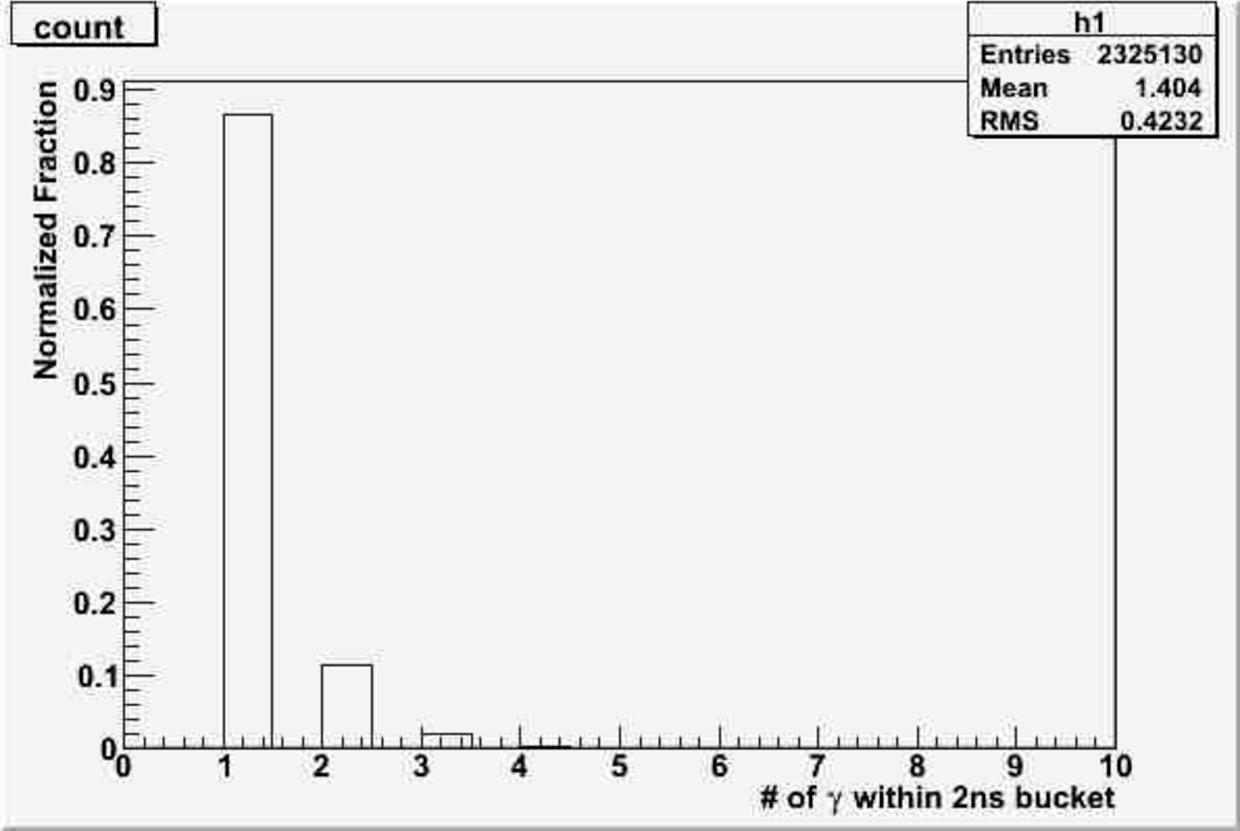
\includegraphics[width=\figwidth,height=0.75\hfigheight]{\figures/analysis/photon_timing/Photoncount1.pdf}
\caption[Probability of single and multiple photons within the \abbr{CEBAF} timing window of 2.004~ns]{\label{fig:beam.timing}Probability of single and multiple photons within the \abbr{CEBAF} timing window of 2.004~ns.}
\end{center}\end{figure}

\begin{figure}[h!]\begin{center}
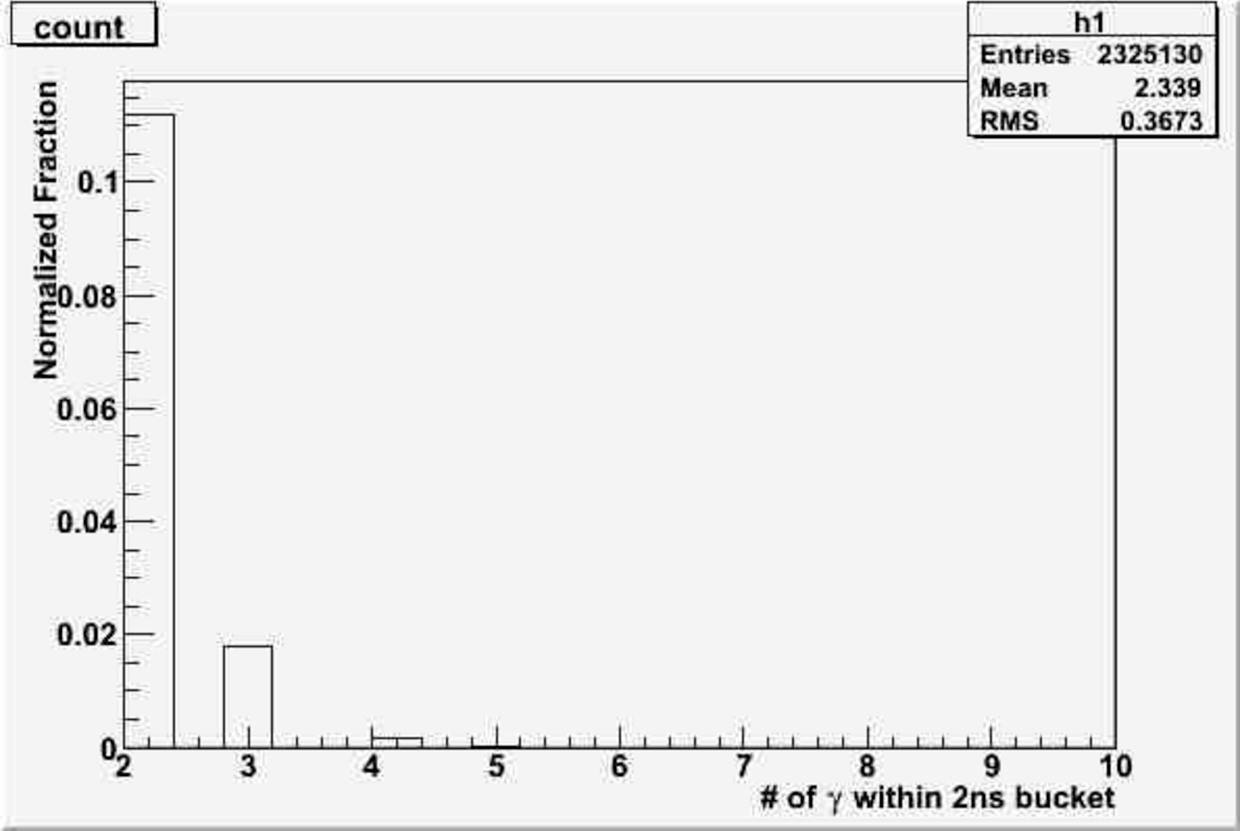
\includegraphics[width=\figwidth,height=0.75\hfigheight]{\figures/analysis/photon_timing/Photoncount.pdf}
\caption[Probability of multiple photons within the \abbr{CEBAF} timing window of 2.004~ns]{\label{fig:beam.timingII}Probability of multiple photons within the \abbr{CEBAF} timing window of 2.004~ns.}
\end{center}\end{figure}

\FloatBarrier
\subsection{Particle Identification}\label{sec:analysis.pid}

Lepton identification was based on conservation of mass. Once the data is skimmed according to Table~\ref{tab:skim.requirements}, all particles that were $\pi^+$, $\pi^-$, unknown with $q^+$ or unknown with $q^-$ were tentatively assigned to be electrons or positrons based on their charge. This meant that the mass term of the particle's 4-vector was set to be the mass of an electron instead of that of a pion. This technique works because the mass of the \piz (0.135~GeV) is less than the mass of $\pi^+$ or $\pi^-$ (0.139~GeV) and by laws of conservation of energy-momentum, a lighter particle cannot decay into heavier particle's.
%To explain this effect, lets consider a particle A decaying into daughters B and C.
%\begin{align}
%A\rightarrow B+C
%\end{align}
%In the rest frame of A the 4-momentum transforms to  
%\begin{align}
%P_A\rightarrow (0,M_A), \nonumber \\
%P_B\rightarrow (\overline{P}_B,E_B), \nonumber \\
%P_C\rightarrow (\overline{P}_C,E_C),
%\end{align}
%where $\overline{P}_B$ and $\overline{P}_C$ are the 3-momentum of particles B and C respectively. Using conservation of 4-momentum and the property $P_i^2 = m_i^2$, $E_C$ can be calculated as;
%\begin{align}\label{eq:piz.kinematics}
%P_B^2 = (P_A - P_C)^2 \nonumber \\
%M_B^2 = P_A^2 + P_C^2 - 2P_A\cdot P_C \nonumber \\
%M_B^2 = M_A^2 + M_C^2 - 2M_AE_C \nonumber \\
%E_C = \frac{M_A^2 + M_C^2 - M_B^2}{2M_A}.
%\end{align}
%For the case in which particle A is a \piz and the particles B and C are electron and positron which have equal mass eq.~\ref{eq:piz.kinematics} simplifies to 
%\begin{align}\label{eq:piz.decay}
%E_C = \frac{M_{\pi^0}^2}{2}.
%\end{align}
%The same procedure can be applied for particle B which would yield the same result as eq.~\ref{eq:piz.decay} with the interchange of the index $C\leftrightarrow B$. From eq.~\ref{eq:piz.decay} it can be seen that because 
%\begin{align}\label{eq:piz.energy}
%E_{C,B} = \sqrt{M_{C,B}^2 + \overline{P}_{C,B}^2} \nonumber
%\end{align}
%that
%\begin{align}
%M_{C,B} <  \frac{M_{\pi^0}^2}{2}, \nonumber
%\end{align}
%therefore \piz cannot decay into particles of heavier mass.

For particles with higher masses that can decay into two-pions  or into \epem, such as $\eta,\ \omega$, etc., the \abbr{CC} and \abbr{EC} provide a $\frac{e^+e^-}{\pi^+\pi^-}$ rejection factor of $\approx 10^6$. The method to achieve this rejection factor was developed by Mike Wood and is based on using various cuts placed on the \abbr{CC} and \abbr{EC} measured quantities. This method was not used in this analysis, the $\gamma p \to  p \pi^0 \to p e^+e^-\gamma$ reaction provides insight into the validity of the method. The Mike Wood method of $\frac{e^+e^-}{\pi^+\pi^-}$ rejection factor is discussed in~\cite{clas.g12.note}.   


%\section{General Features of Lepton Data in \g12}\label{sec:analysis.Lepton.general}

Electron and positron energy deposition while propagating through a material was briefly explained in Sec.~\ref{sec:clas.cc} and ~\ref{sec:clas.ec}. To identify electrons and positrons properly in \abbr{CLAS}, quantities obtained from the \abbr{CC} and \abbr{EC} are used to reject charged pions. The \abbr{CC} collects the number of photo-electrons caused by Cherenkov radiation and the \abbr{EC} records the energy deposition of electrons/positrons as well as photons. A previous \abbr{CLAS} experiment \emph{g7} analyzed the properties of medium modifications from the decay of vector mesons through the leptonic decay channel. This experiment derived a set of cits for identifying electron/positrons pairs in \abbr{CLAS} by employing specific cuts to the number of photo-electrons (\abbr{NPE}) detected in the \abbr{CC}, a match in azimuthal angle $\phi$ from a charged track in the \abbr{DC} to the $\phi$ of the \abbr{CC}, as well as comparing the momentum of the charged track to the energy deposited in the \abbr{EC}. These cuts can be found in Table~\ref{tab:ISLEP_cuts}.  
\begin{table}[h!]
\begin{minipage}{\textwidth}
\begin{center}
\begin{singlespacing}

\caption[Electron/Positron PID Cuts]{\label{tab:ISLEP_cuts}Cuts applied to the \abbr{CC} and \abbr{EC} to perform electron/positron \abbr{PID} \vspace{0.75mm}}

\begin{tabular}{c|c|c}

\hline
Subsystem & Quantity & Cut \\
\hline
\multirow{2}{*}{\abbr{CC}}  & \# of photo-electrons (\abbr{NPE})  & \abbr{NPE} $>$ 2.5 \\
 &  \abbr{DC} $\phi$ \& \abbr{CC} $\phi$  & \abbr{DC} $\phi$ = \abbr{CC} $\phi$ \\
\hline
\multirow{2}{*}{\abbr{EC}}  & q$^{\pm}$ momentum threshold (p$\mathrm{_{thres}}$) & \multirow{2}{*}{p$\mathrm{_{thres}^{high}} < \ $E$\mathrm{_{calo}} <$ p$\mathrm{_{thres}^{low}}$ } \\
&  \& \abbr{EC} deposited energy (E$\mathrm{_{calo}}$) & \\
\hline \hline
\end{tabular}

%\begin{tabular}{c|c|c}
%\hline
%Subsystem & Quantity & Cut   \vspace{0.5mm} \\
%\hline
%\multirow{2}{*}{\abbr{CC}}  & \# of photo-electrons (\abbr{NPE})  & \abbr{NPE} $>$ 2.5 \\
% &  \abbr{DC} $\phi$ \& \abbr{CC} $\phi$  & \abbr{DC} $\phi$ = \abbr{CC} $\phi$ \\
%\hline
% \multirow{2}{*}{\abbr{EC}}  & q$^{\pm}$ momentum threshold (p$\mathrm{_{thres}}$) \& \abbr{EC} deposited energy (E$\mathrm{_{calo}}$)& p$\mathrm{_{thres}^{low}}$ $<$E$\mathrm{_{calo}}$ \\
%  &  q$^{\pm}$ momentum \& \abbr{EC} deposited energy  & \abbr{DC} $\phi$ = \abbr{CC} $\phi$ \\
%\hline \hline
%\end{tabular}  


\end{singlespacing}
\end{center}
\end{minipage}
\end{table}
\vspace{20pt}
To validate the \emph{g7} electron/positron \abbr{PID} scheme for \g12, a comparison of  the \abbr{CC} and \abbr{EC} quantities was performed for all charged tracks \abbr{CC}/\abbr{EC} hit signatures and while selecting events from \piz decay. To separate the \piz events from the $\pi^{+}\pi^{-}$ events, all charged pions were assigned the mass of electrons and cuts were placed on the missing energy of $\gamma p \rightarrow p e^+ e^-$ as well as a cut on the missing mass squared of $\gamma p \rightarrow p$, values found in Table~\ref{tab:lep_cuts}. A graphical depiction of the cuts applied to separate \piz events from the $\pi^{+}\pi^{-}$ events is seen in Fig.~\ref{fig:islep.cuts}.
\begin{table}[h!]
\begin{minipage}{\textwidth}
\begin{center}
\begin{singlespacing}

\caption[Cuts To Seperate \piz from $\pi^{+}\pi^{-}$ for \abbr{PID} Validation]{\label{tab:lep_cuts}Cuts applied to seperate \piz evetns from $\pi^{+}\pi^{-}$ events \vspace{0.75mm}}

\begin{tabular}{c|c|c}

\hline
Cut Topology & Topology Quantity & Value  \\
\hline
$\gamma p \rightarrow p e^+ e^-$ & Missing Energy ($\mathrm{M_E}$) & $>0.075$~GeV \\
\hline
\multirow{2}{*}{$\gamma p \rightarrow p $}  & \multirow{2}{*}{Missing mass squared ($\mathrm{M_x^2}$)} & $<$ 0.0779~GeV$^2$ for \piz events \\
&  & $>$ 0.0779~GeV$^2$ for $\pi^{+}\pi^{-}$ events\\
\hline \hline
\end{tabular}

\end{singlespacing}
\end{center}
\end{minipage}
\end{table}
\vspace{20pt} 
The values of the threshold momentum are calculated from empirical studies and are based upon calculations using the momentum obtained from the \abbr{DC }$p$ under the following criteria;
\begin{align}
\mathrm{p_{thres}^{low}} = \alpha p *(p+EC_{P\_LO})/p \nonumber \\
\mathrm{p_{thres}^{high}} = \alpha p *(p+EC_{P\_HIGH})/p \nonumber
\end{align}
where $EC_{P\_LO} = -0.3$, $EC_{P\_HIGH} = 0.5$ and  
\begin{align}
\alpha p =
\begin{cases}
.23*p + .071p^2 - .032p^3, & p<1.0 \mathrm{~GeV} \\
0.272p, & p>1.0 \mathrm{~GeV} \\
\end{cases}\nonumber
\end{align}


\begin{figure}[h!]\begin{center}
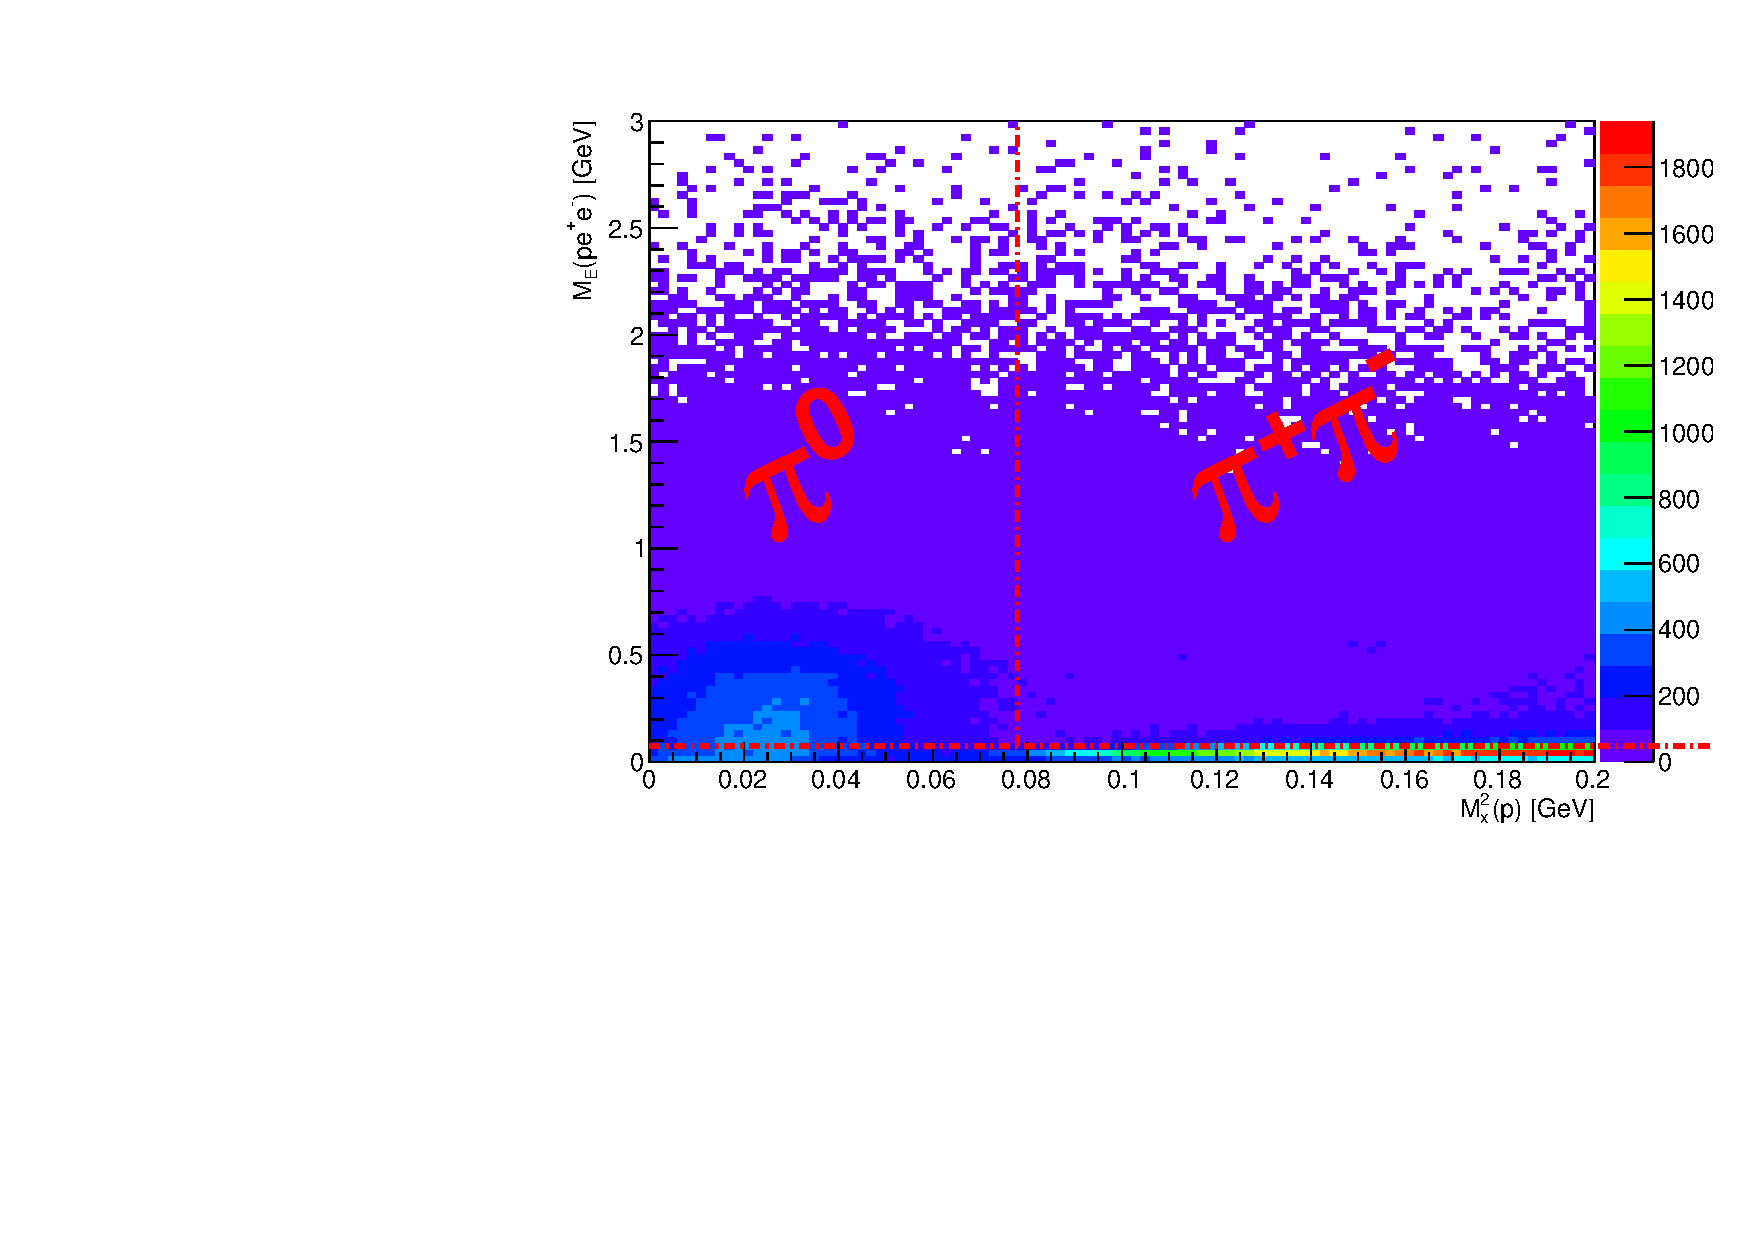
\includegraphics[width=\figwidth,height=\hfigheight]{\figures/analysis/LEP_FEATURES/Lepfeature_cuts.pdf}
\caption[Cuts Applied to Isolate \piz and $\pi^{+}\pi^{-}$ for \abbr{PID} Validation]{\label{fig:islep.cuts}Plot of missing mass squared of off proton (horizontal) vs. missing energy of proton e$^+$e$^-$ (vertical). The red dashed vertical line depicts the $\pi^{+}\pi^{-}$ threshold mass cut while the horizontal red dashed line represents the missing energy cut-off used to sepertate $\pi^{+}\pi^{-}$ from \piz.}
\end{center}\end{figure}

\subsubsection{\abbr{CC} Comparison}

The \abbr{NPE} measured by the \abbr{CC} for all positron/electron (e$^+$/e$^-$) candidates can be seen in Fig~\ref{fig:islep.CC}. The sharp decline prior to 2.5 \abbr{NPE} is due to photo-electrons created by electron/positrons, pions traveling through the \abbr{CC} or pions producing delta-electrons which pass through the \abbr{CC}. Delta-electrons are created as an effect of the ionization of gases that could be present when the pion travels through the \abbr{DC}. These types of electrons are typically lower in momentum than the electrons obtained from particle decays in \abbr{CLAS} and thus according to eq.~\ref{eq:cc.NPE} should emit less \abbr{NPE} per unit length.

Through mass conservation, as discussed in Sec.~\ref{sec:analysis.pid}, the particles in the \piz events must be e$^+$/e$^-$ pairs. In comparison to fig.~\ref{fig:islep.CC}, fig.~\ref{fig:islep.CC1} plots the \abbr{NPE} measured by the \abbr{CC} for all e$^+$/e$^-$ pairs for \piz events selected as shown in fig.~\ref{fig:islep.cuts}. It can be seen that the sharp decline prior to \abbr{NPE} = 2.5 is reduced leaving mostly electrons or positrons signatures in the \abbr{CC} concluding that the \emph{g7} \abbr{CC} \abbr{NPE} cut is valid for identifying e$^+$/e$^-$ pairs while rejecting $\pi^+$/$\pi^-$ pairs.
 
%
\begin{figure}[h!]\begin{center}
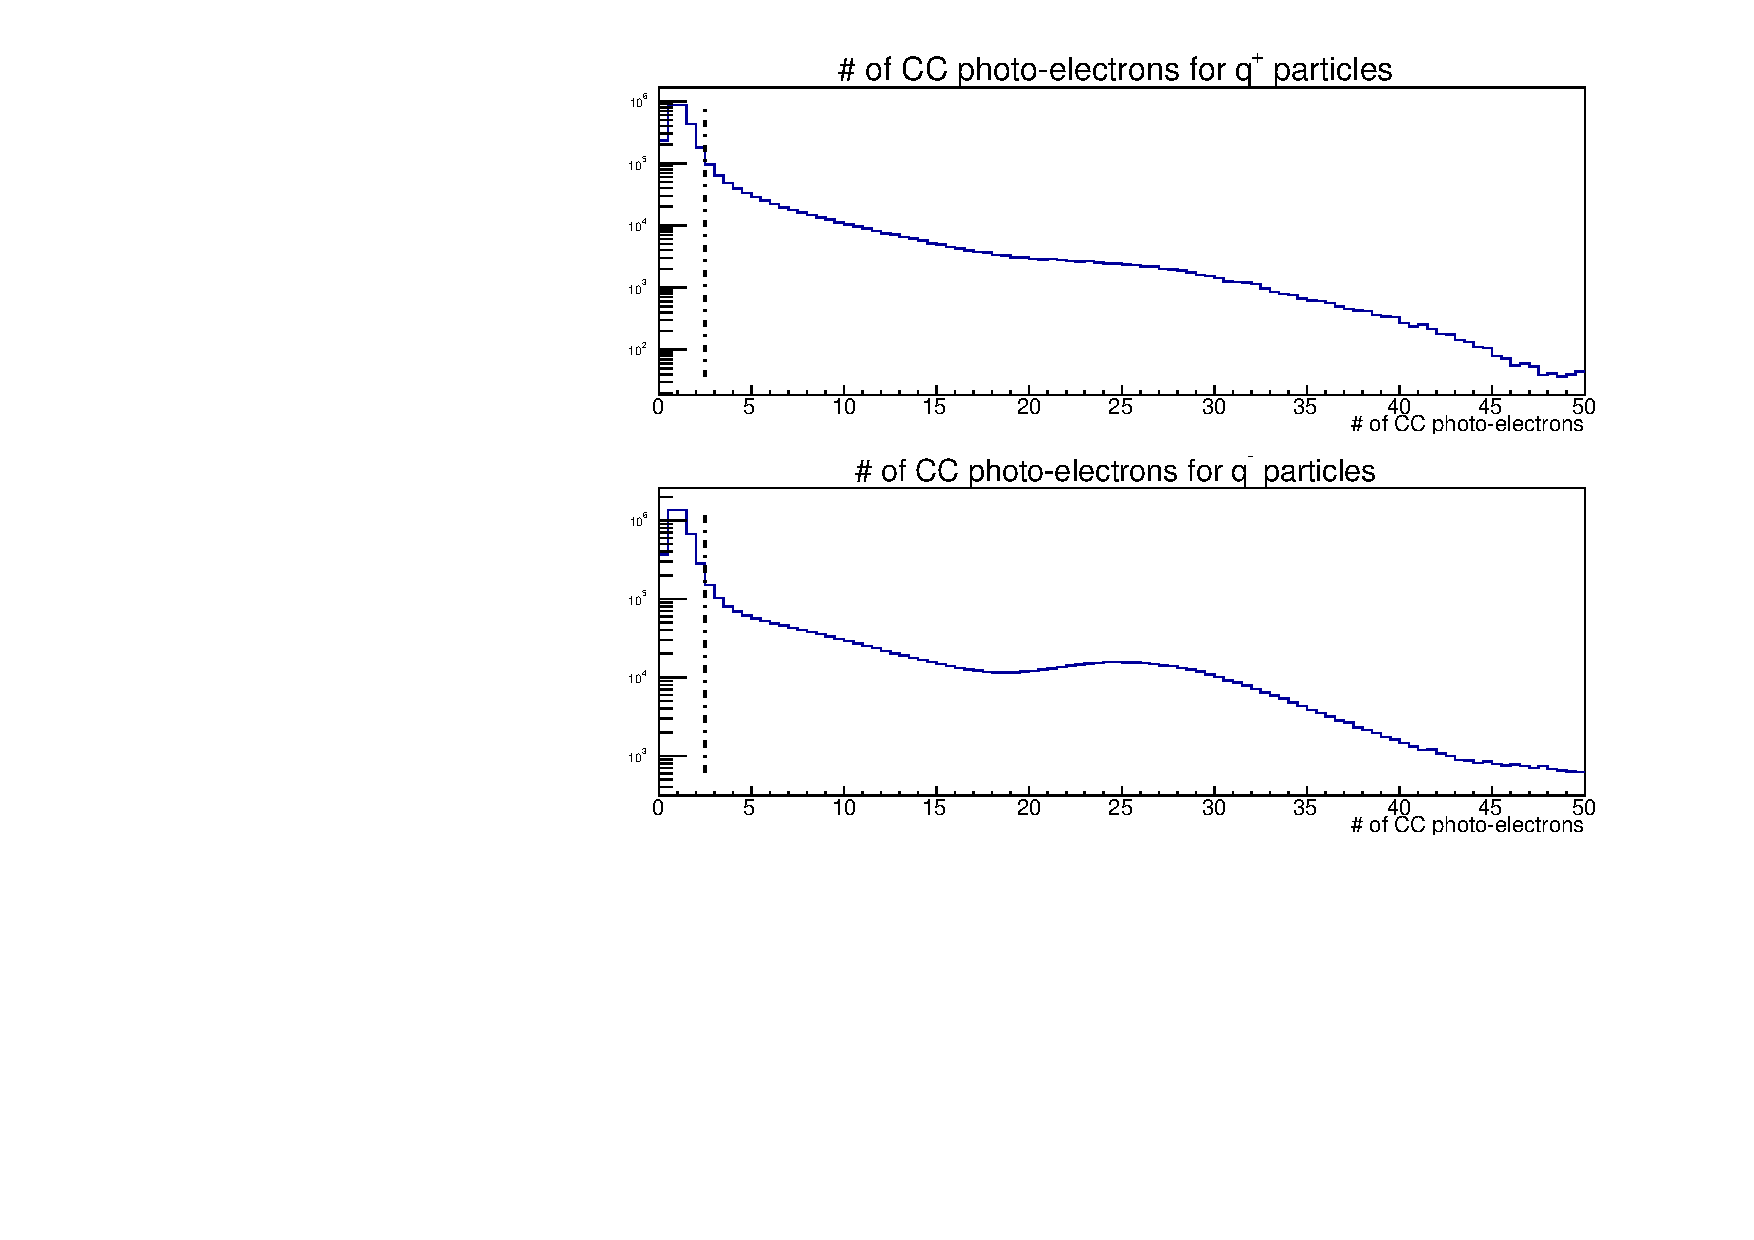
\includegraphics[width=\figwidth,height=\hfigheight]{\figures/analysis/LEP_FEATURES/CC_nPE.pdf}
\caption[Number of Photo-electrons Measured by \abbr{CC} for All e$^-$ and e$^+$ Candidates]{\label{fig:islep.CC}Plot of \abbr{NPE} measured by \abbr{CLAS} \abbr{CC} subsystem for positron/electron candidates top/bottom respectively. The dashed dotted vertical line depicts the cut applied if using the \emph{g7} lepton \abbr{PID} scheme.}
\end{center}\end{figure}

\begin{figure}[h!]\begin{center}
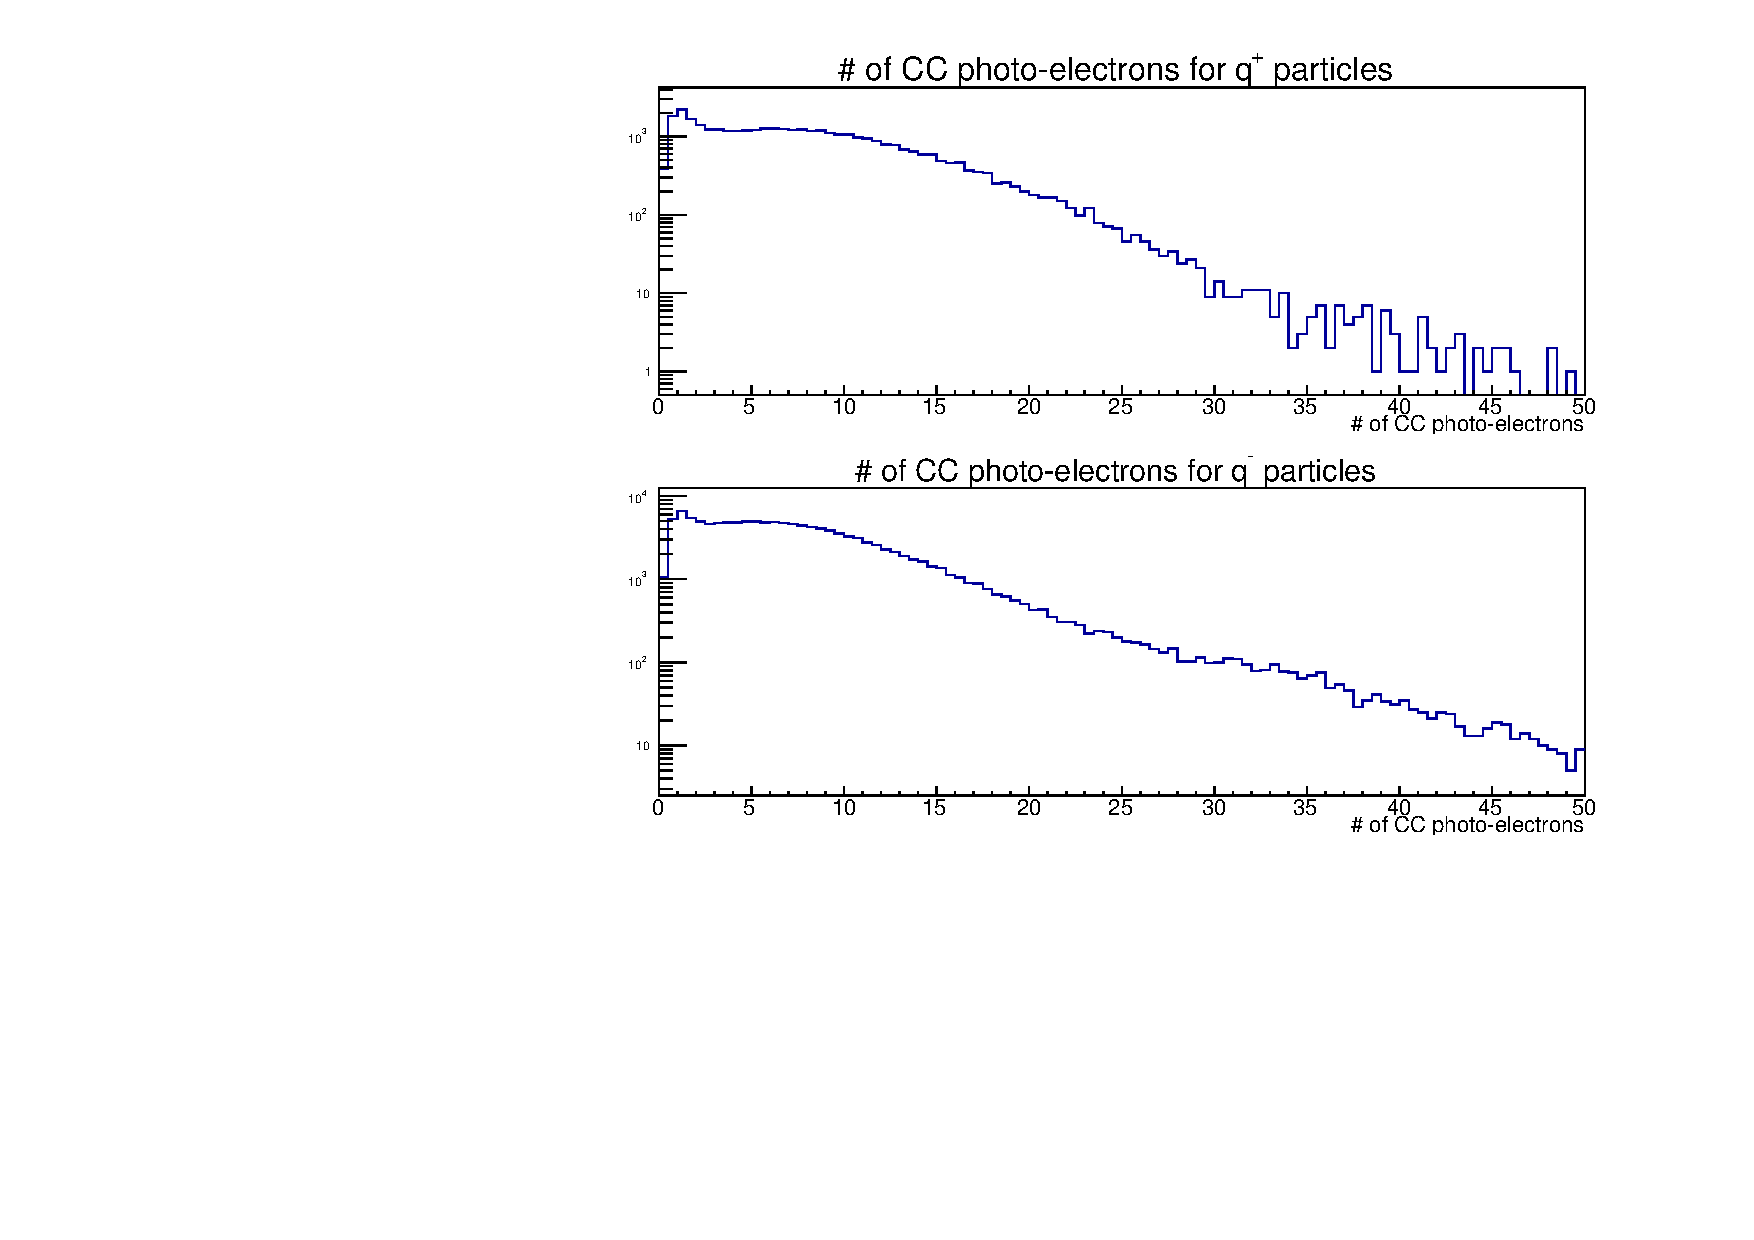
\includegraphics[width=\figwidth,height=\hfigheight]{\figures/analysis/LEP_FEATURES/CC_NPEcut.pdf}
\caption[Number of Photo-electrons Measured by \abbr{CC} for \piz Events]{\label{fig:islep.CC1}Plot of \abbr{NPE} measured by \abbr{CLAS} \abbr{CC} subsystem when selecting \piz events seen in Fig~\ref{fig:islep.cuts}, positron/electron candidates top/bottom respectively.}
\end{center}\end{figure}
\FloatBarrier
\subsubsection{\abbr{EC} Comparison}
%EC
%
%e-
%

Similarly to the \abbr{CC} comparison, figures~\ref{fig:islep.pimEClow},~\ref{fig:islep.pimEChigh},~\ref{fig:islep.pipEClow},~\ref{fig:islep.pipEChigh} depict the  p$\mathrm{_{thres}^{low}}$ and  p$\mathrm{_{thres}^{low}}$ cuts listed in  Table~\ref{tab:ISLEP_cuts} for the q$^-$ and q$^+$ tracks respectively. After \piz event selection, seen in figures~\ref{fig:islep.pimEC},~\ref{fig:islep.pimECcut} ,~\ref{fig:islep.pipEC} ,~\ref{fig:islep.pipECcut}, the bulk of e$^+$/e$^-$ events reside within the region of the cut acceptance therefore it is evident that the \emph{g7} \abbr{EC} cuts are valid for identifying e$^+$/e$^-$ pairs. The following four plots are for electron($e^-$) \abbr{PID} validation of the \emph{g7} \abbr{EC} cuts described in Table~\ref{tab:ISLEP_cuts}.
%
\begin{figure}[h!]\begin{center}
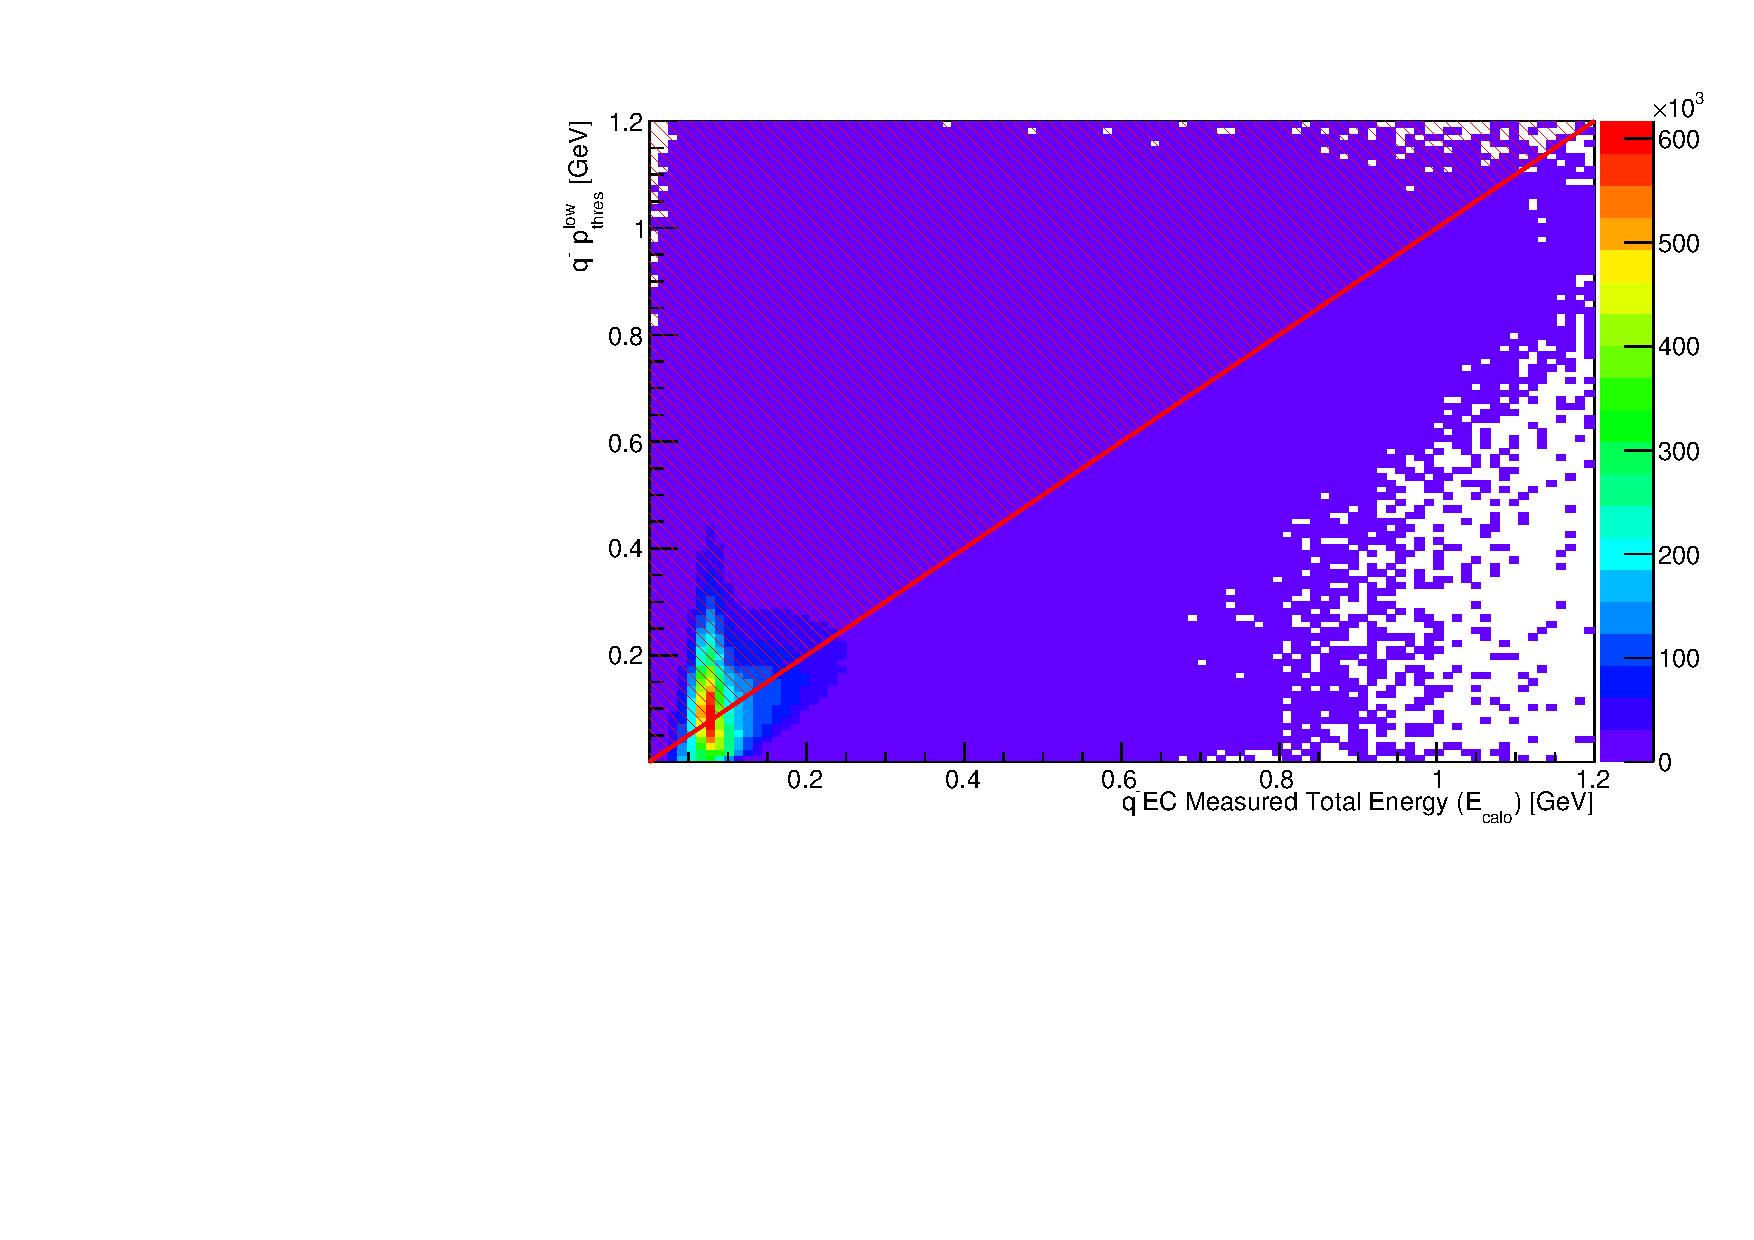
\includegraphics[width=\figwidth,height=0.7\hfigheight]{\figures/analysis/LEP_FEATURES/Pim_EClow.pdf}
\caption[\abbr{EC} Deposited Energy Comparison to Lower Threshold Track Momentum for q$^-$ Tracks]{\label{fig:islep.pimEClow}Plot of energy deposited measured by \abbr{EC} vs. track momentum p$\mathrm{_{thres}^{low}}$ for negative charged tracks. The red region depicts the cut that would reject events in the \emph{g7} lepton \abbr{EC} \abbr{PID} scheme.}
\end{center}\end{figure}

\begin{figure}[h!]\begin{center}
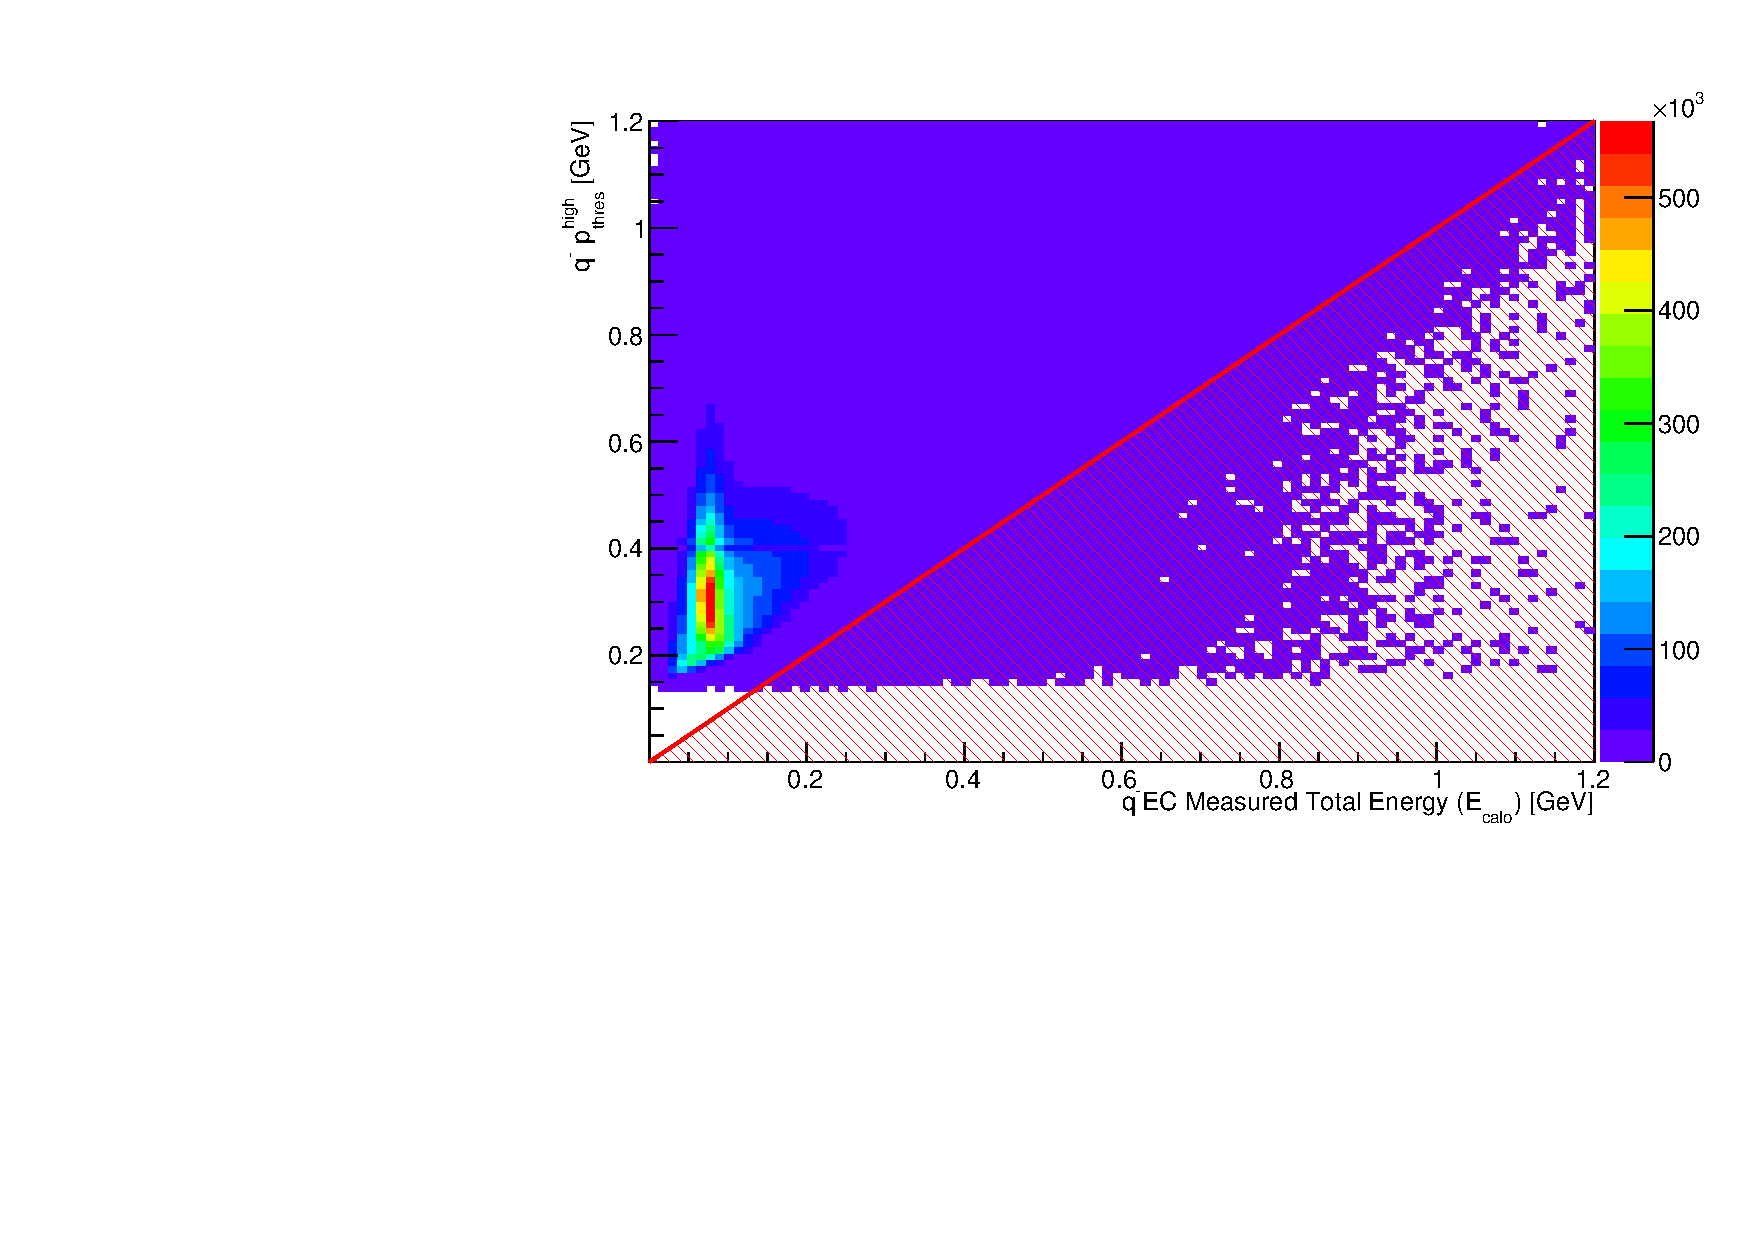
\includegraphics[width=\figwidth,height=0.7\hfigheight]{\figures/analysis/LEP_FEATURES/Pim_EChigh.pdf}
\caption[\abbr{EC} Deposited Energy Comparison to Upper Threshold Track Momentum for q$^-$ Tracks]{\label{fig:islep.pimEChigh}Plot of energy deposited measured by \abbr{EC} vs. track momentum p$\mathrm{_{thres}^{high}}$ for negative charged tracks. The red region depicts the cut that would reject events in the \emph{g7} lepton \abbr{EC} \abbr{PID} scheme.}
\end{center}\end{figure}


\begin{figure}[h!]\begin{center}
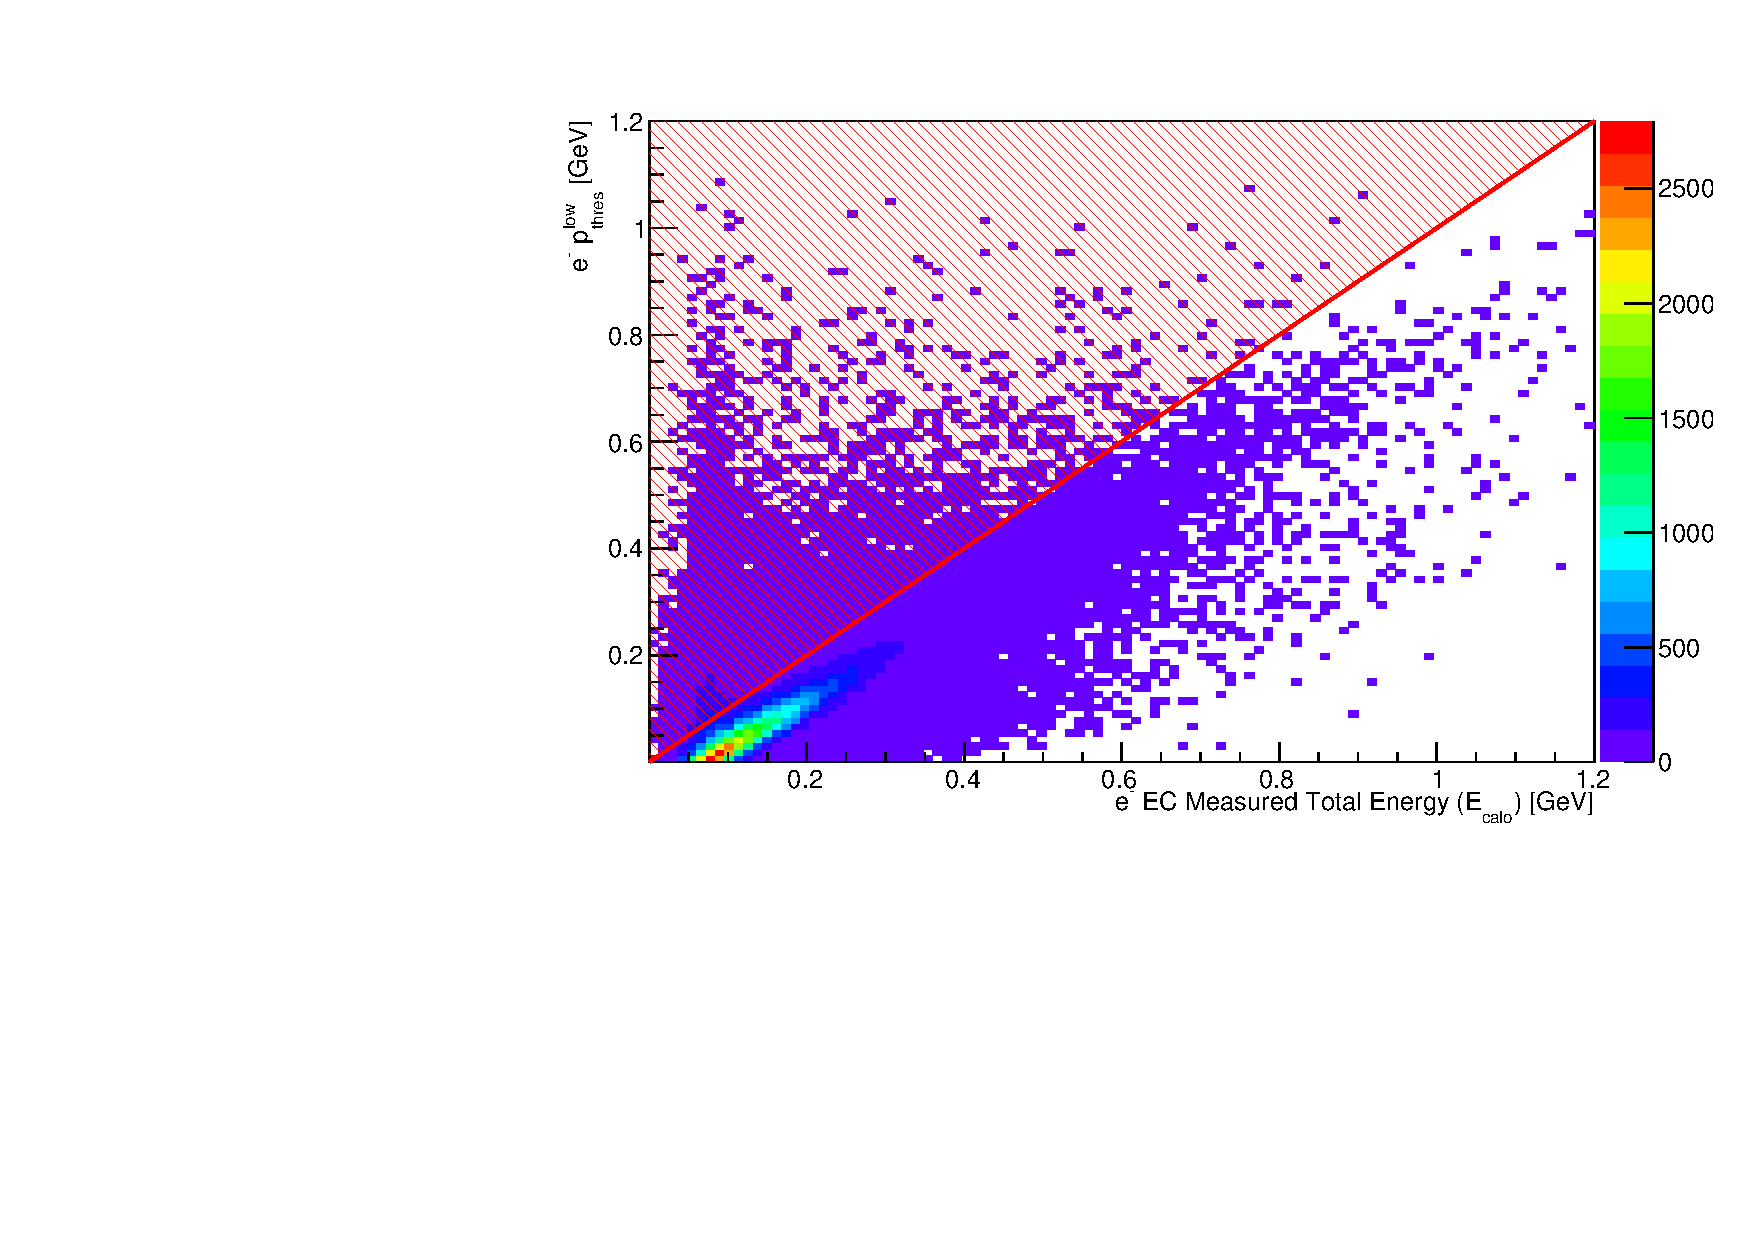
\includegraphics[width=\figwidth,height=0.7\hfigheight]{\figures/analysis/LEP_FEATURES/Pim_EClowcut.pdf}
\caption[\abbr{EC} Deposited Energy Comparison to Track Momentum for e$^-$ Candidates]{\label{fig:islep.pimEC}Plot of energy deposited measured by \abbr{EC} vs. track momentum p$\mathrm{_{thres}^{low}}$ for electrons from \piz events without the \emph{g7} lepton \abbr{EC} \abbr{PID} scheme applied. The red region depicts the cut that would reject events in the \emph{g7} lepton \abbr{EC} \abbr{PID} scheme.}
\end{center}\end{figure}

\begin{figure}[h!]\begin{center}
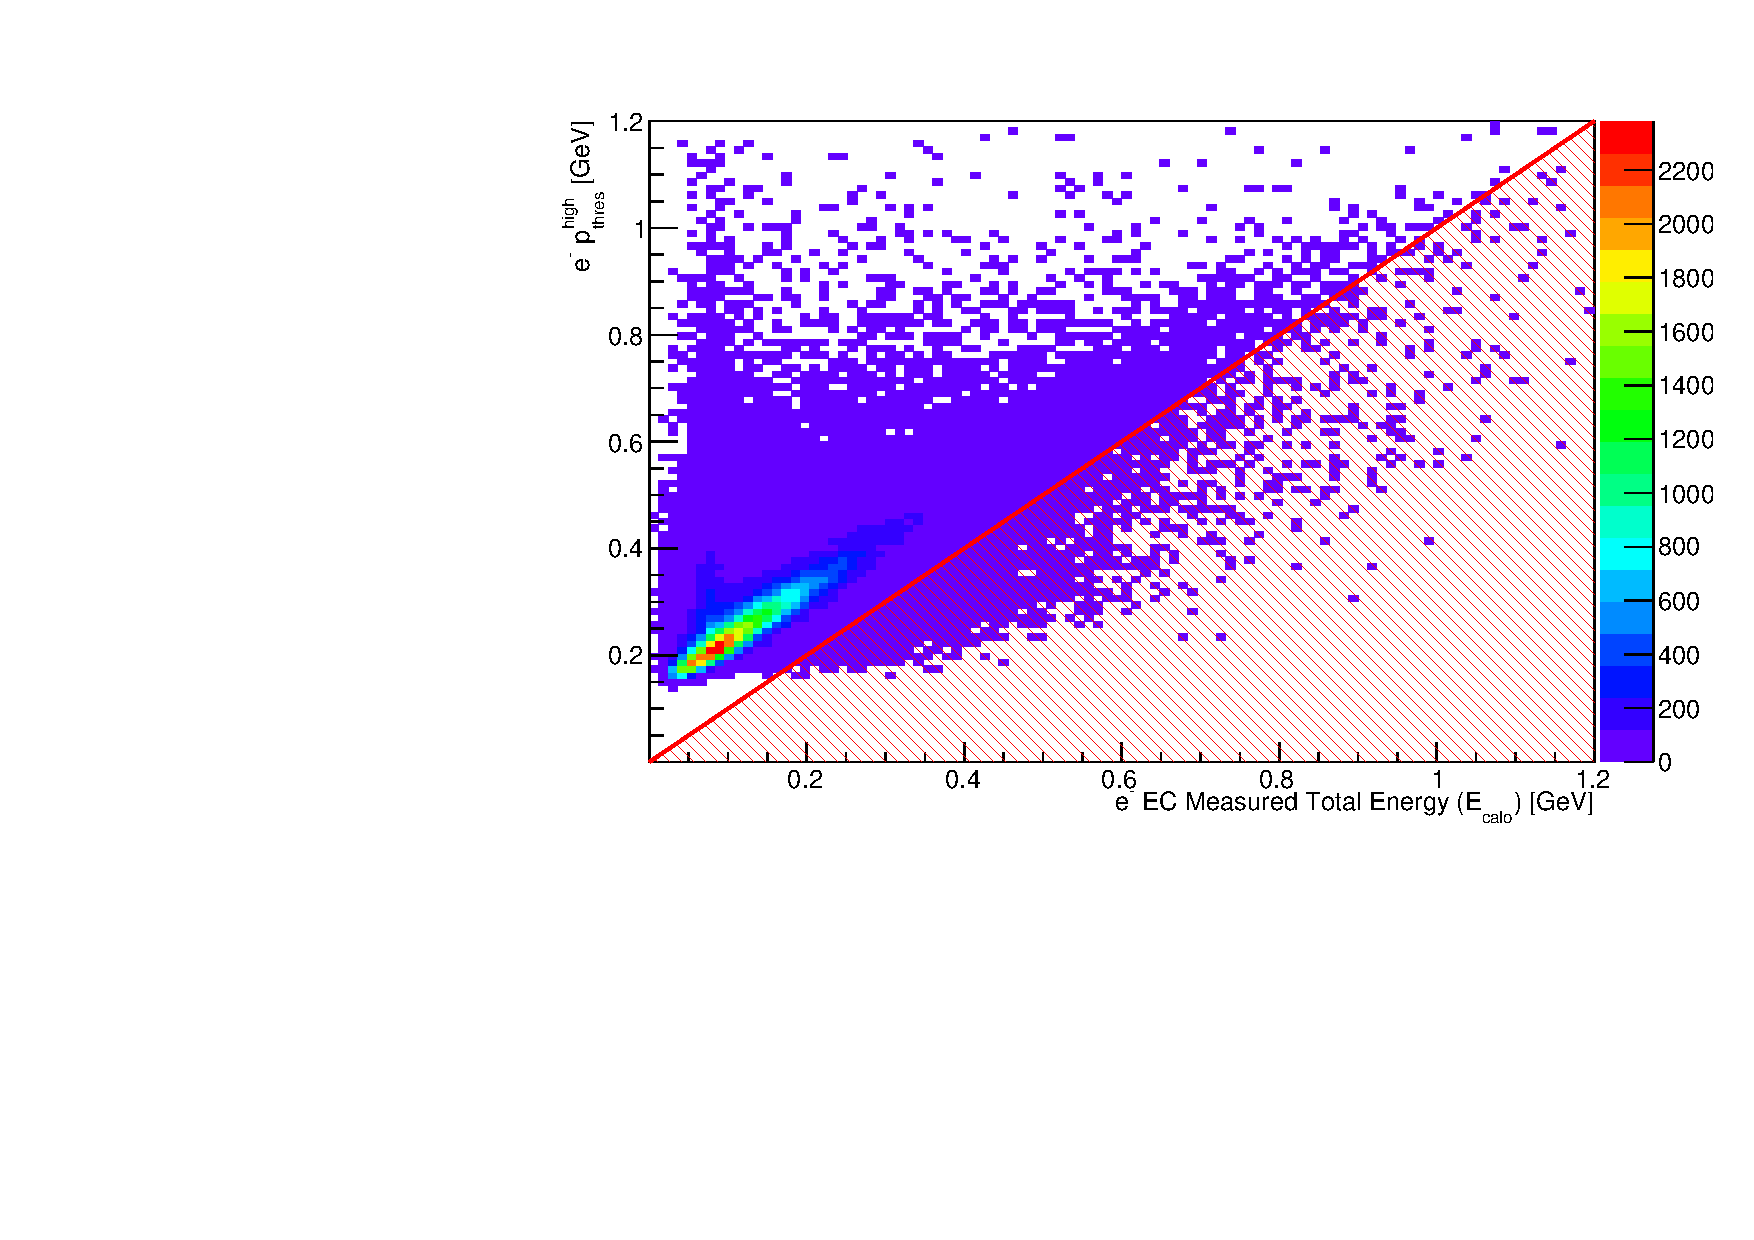
\includegraphics[width=\figwidth,height=0.7\hfigheight]{\figures/analysis/LEP_FEATURES/Pim_EChighcut.pdf}
\caption[\abbr{EC} Deposited Energy Comparison to Track Momentum for e$^-$ from \piz Events]{\label{fig:islep.pimECcut}Plot of energy deposited measured by \abbr{EC} vs. track momentum p$\mathrm{_{thres}^{high}}$ for electrons from \piz events without the \emph{g7} lepton \abbr{EC} \abbr{PID} scheme applied. The red region depicts the cut that would reject events in the \emph{g7} lepton \abbr{EC} \abbr{PID} scheme.}
\end{center}\end{figure}
\FloatBarrier
The following four plots are for positron($e^+$) \abbr{PID} validation of the \emph{g7} \abbr{EC}
cuts described in Table~\ref{tab:ISLEP_cuts}.
%
%
%e+
%
%
\begin{figure}[h!]\begin{center}
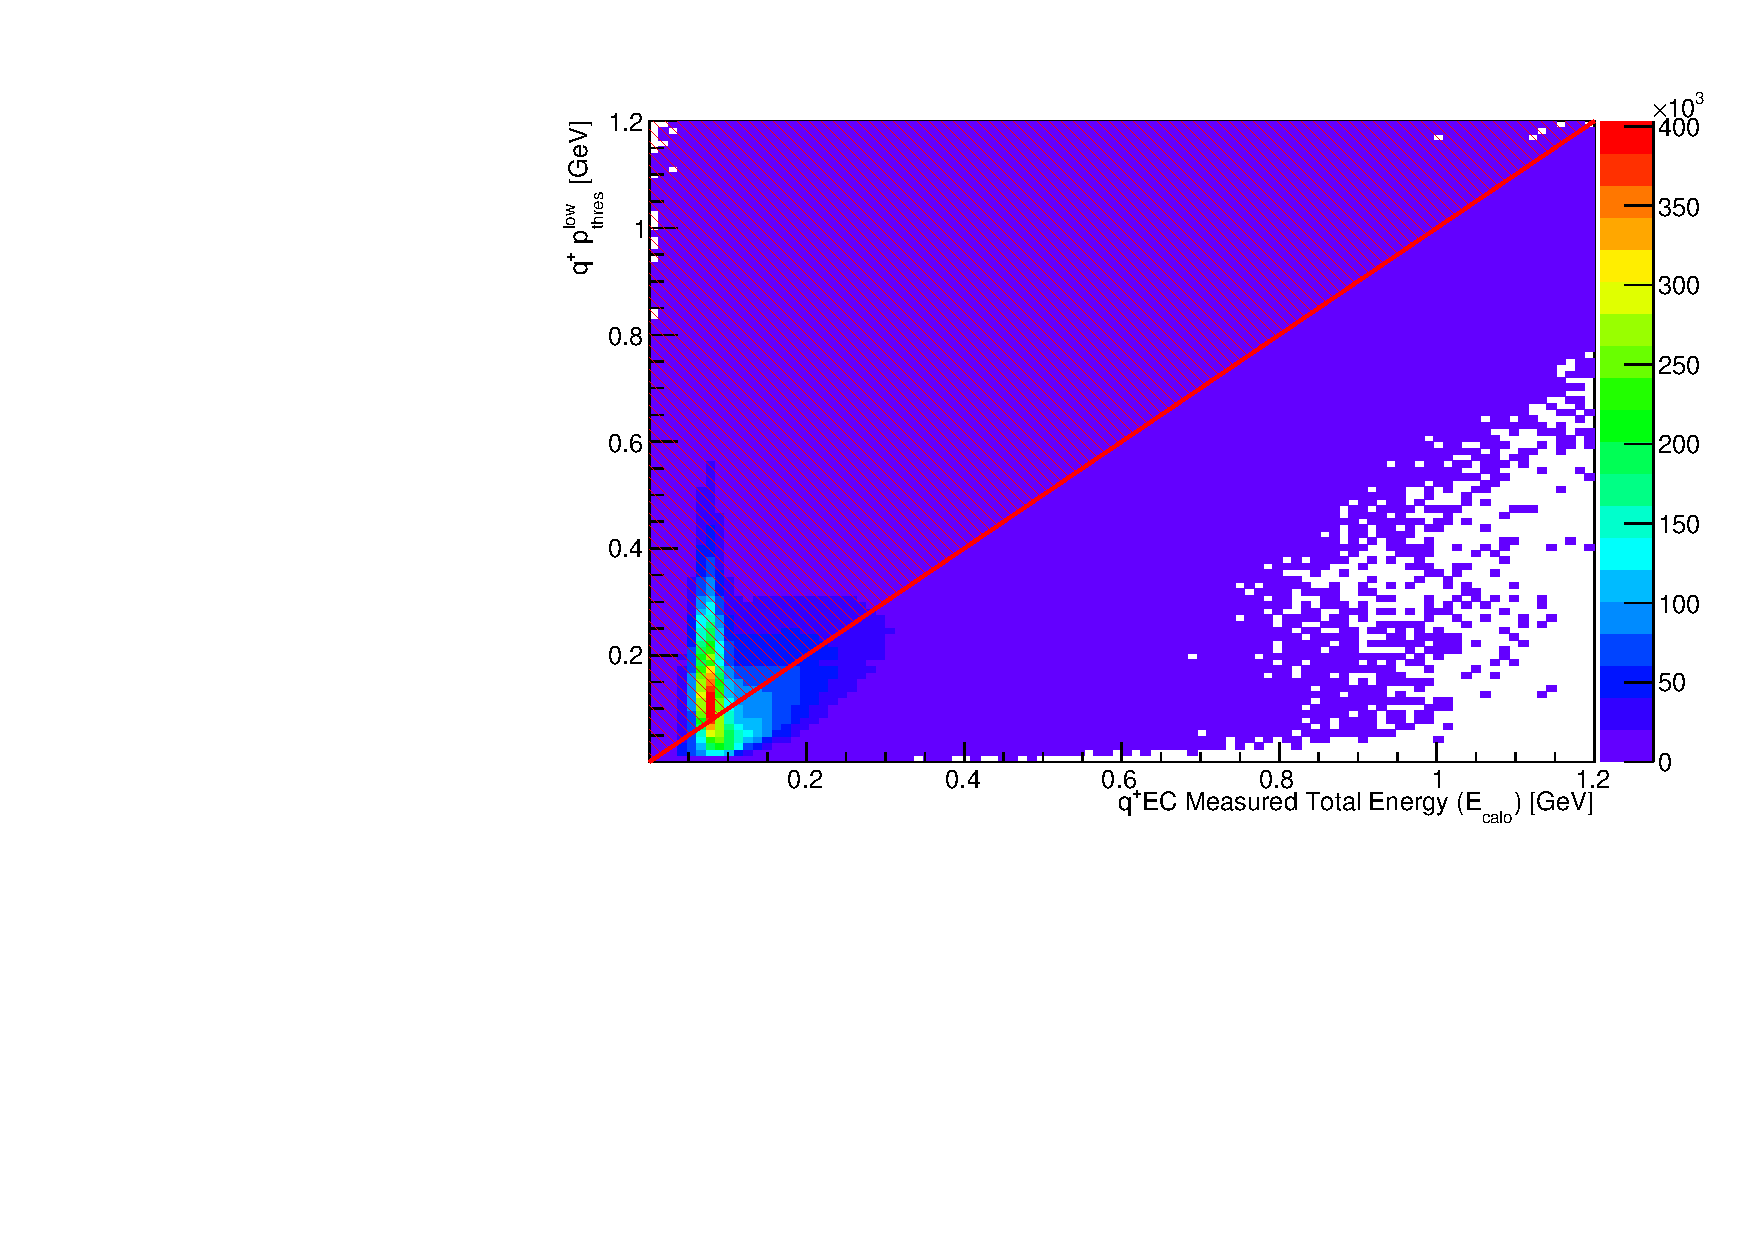
\includegraphics[width=\figwidth,height=0.7\hfigheight]{\figures/analysis/LEP_FEATURES/Pip_EClow.pdf}
\caption[\abbr{EC} Deposited Energy Comparison to Lower Threshold Track Momentum for q$^+$ Tracks]{\label{fig:islep.pipEClow}Plot of energy deposited measured by \abbr{EC} vs. track momentum p$\mathrm{_{thres}^{low}}$ for positive charged tracks. The red region depicts the cut that would reject events in the \emph{g7} lepton \abbr{EC} \abbr{PID} scheme.}
\end{center}\end{figure}

\begin{figure}[h!]\begin{center}
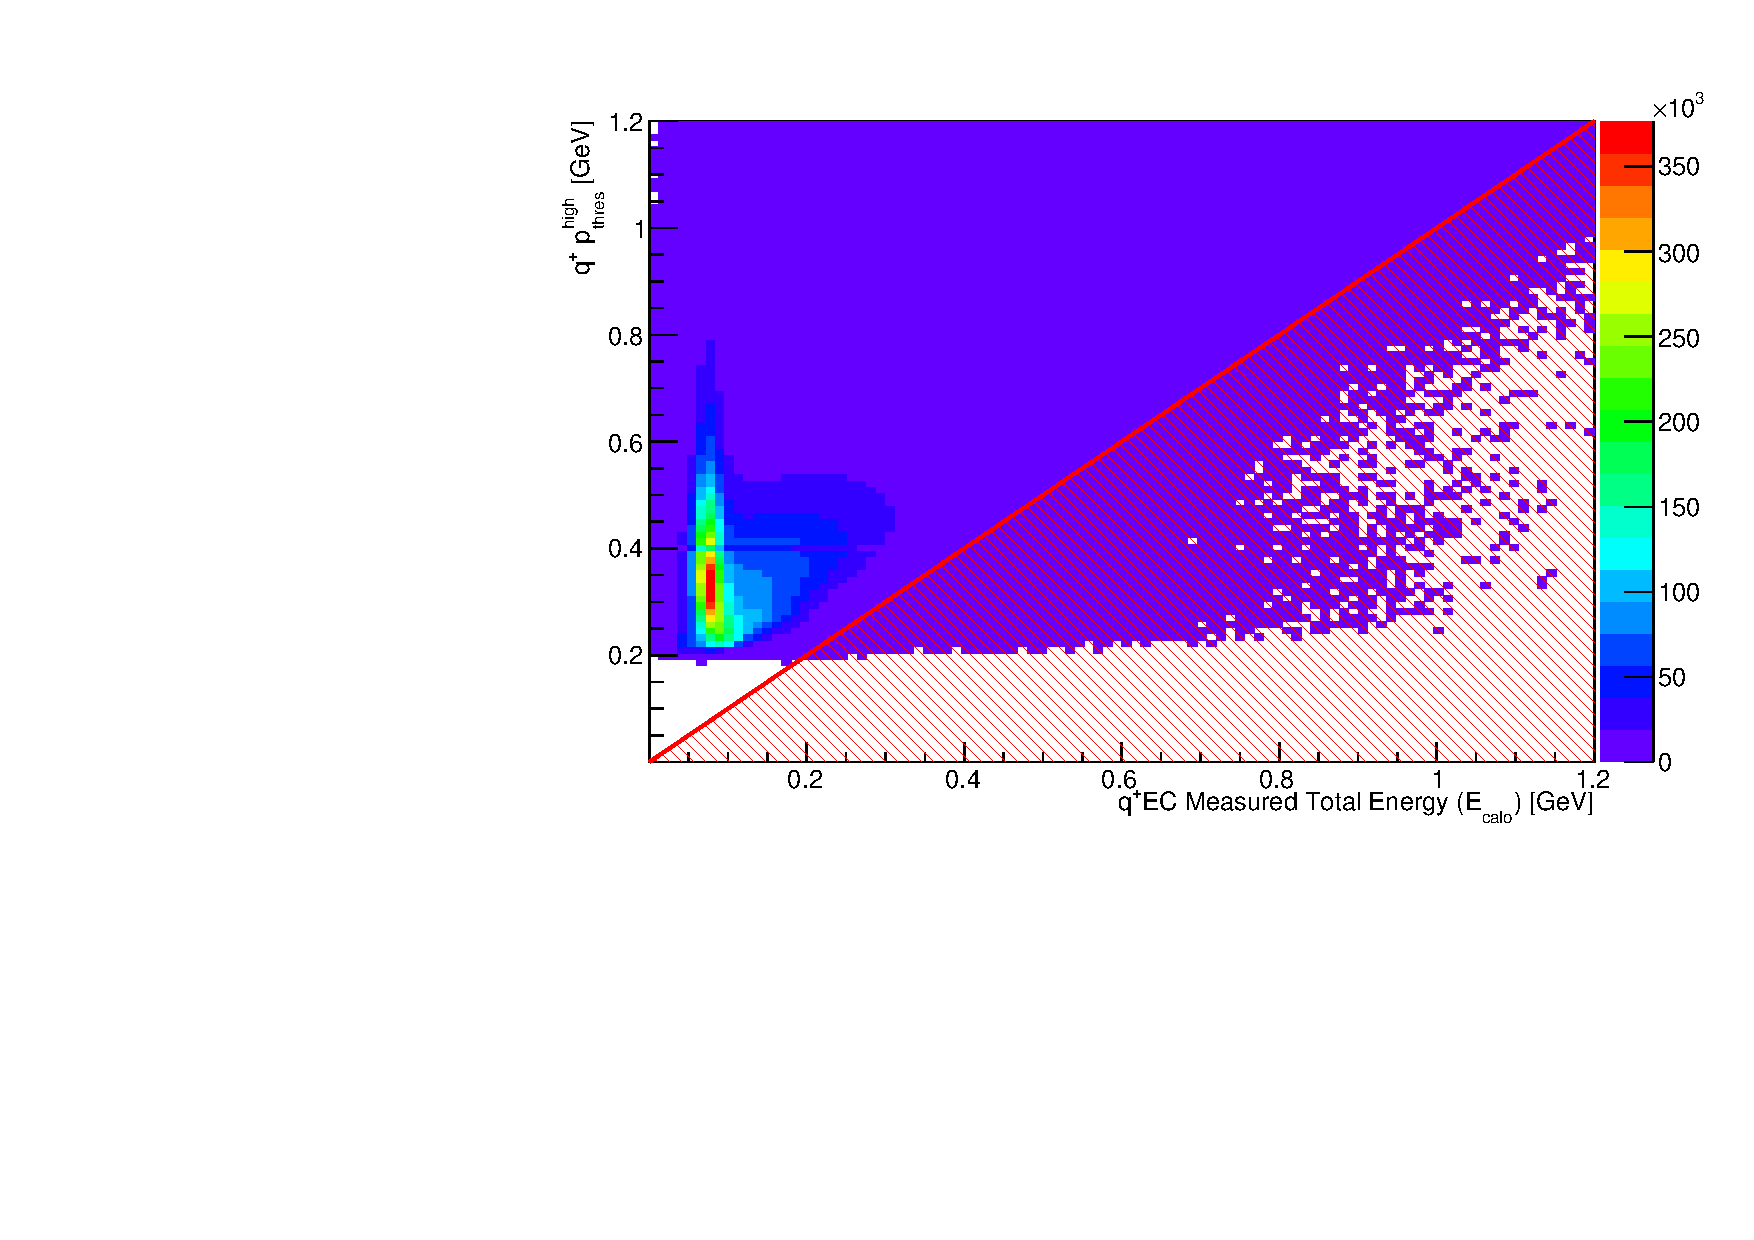
\includegraphics[width=\figwidth,height=0.7\hfigheight]{\figures/analysis/LEP_FEATURES/Pip_EChigh.pdf}
\caption[\abbr{EC} Deposited Energy Comparison to Upper Threshold Track Momentum for q$^+$ Tracks]{\label{fig:islep.pipEChigh}Plot of energy deposited measured by \abbr{EC} vs. track momentum p$\mathrm{_{thres}^{high}}$ for positive charged tracks. The red region depicts the cut that would reject events in the \emph{g7} lepton \abbr{EC} \abbr{PID} scheme.}
\end{center}\end{figure}

\begin{figure}[h!]\begin{center}
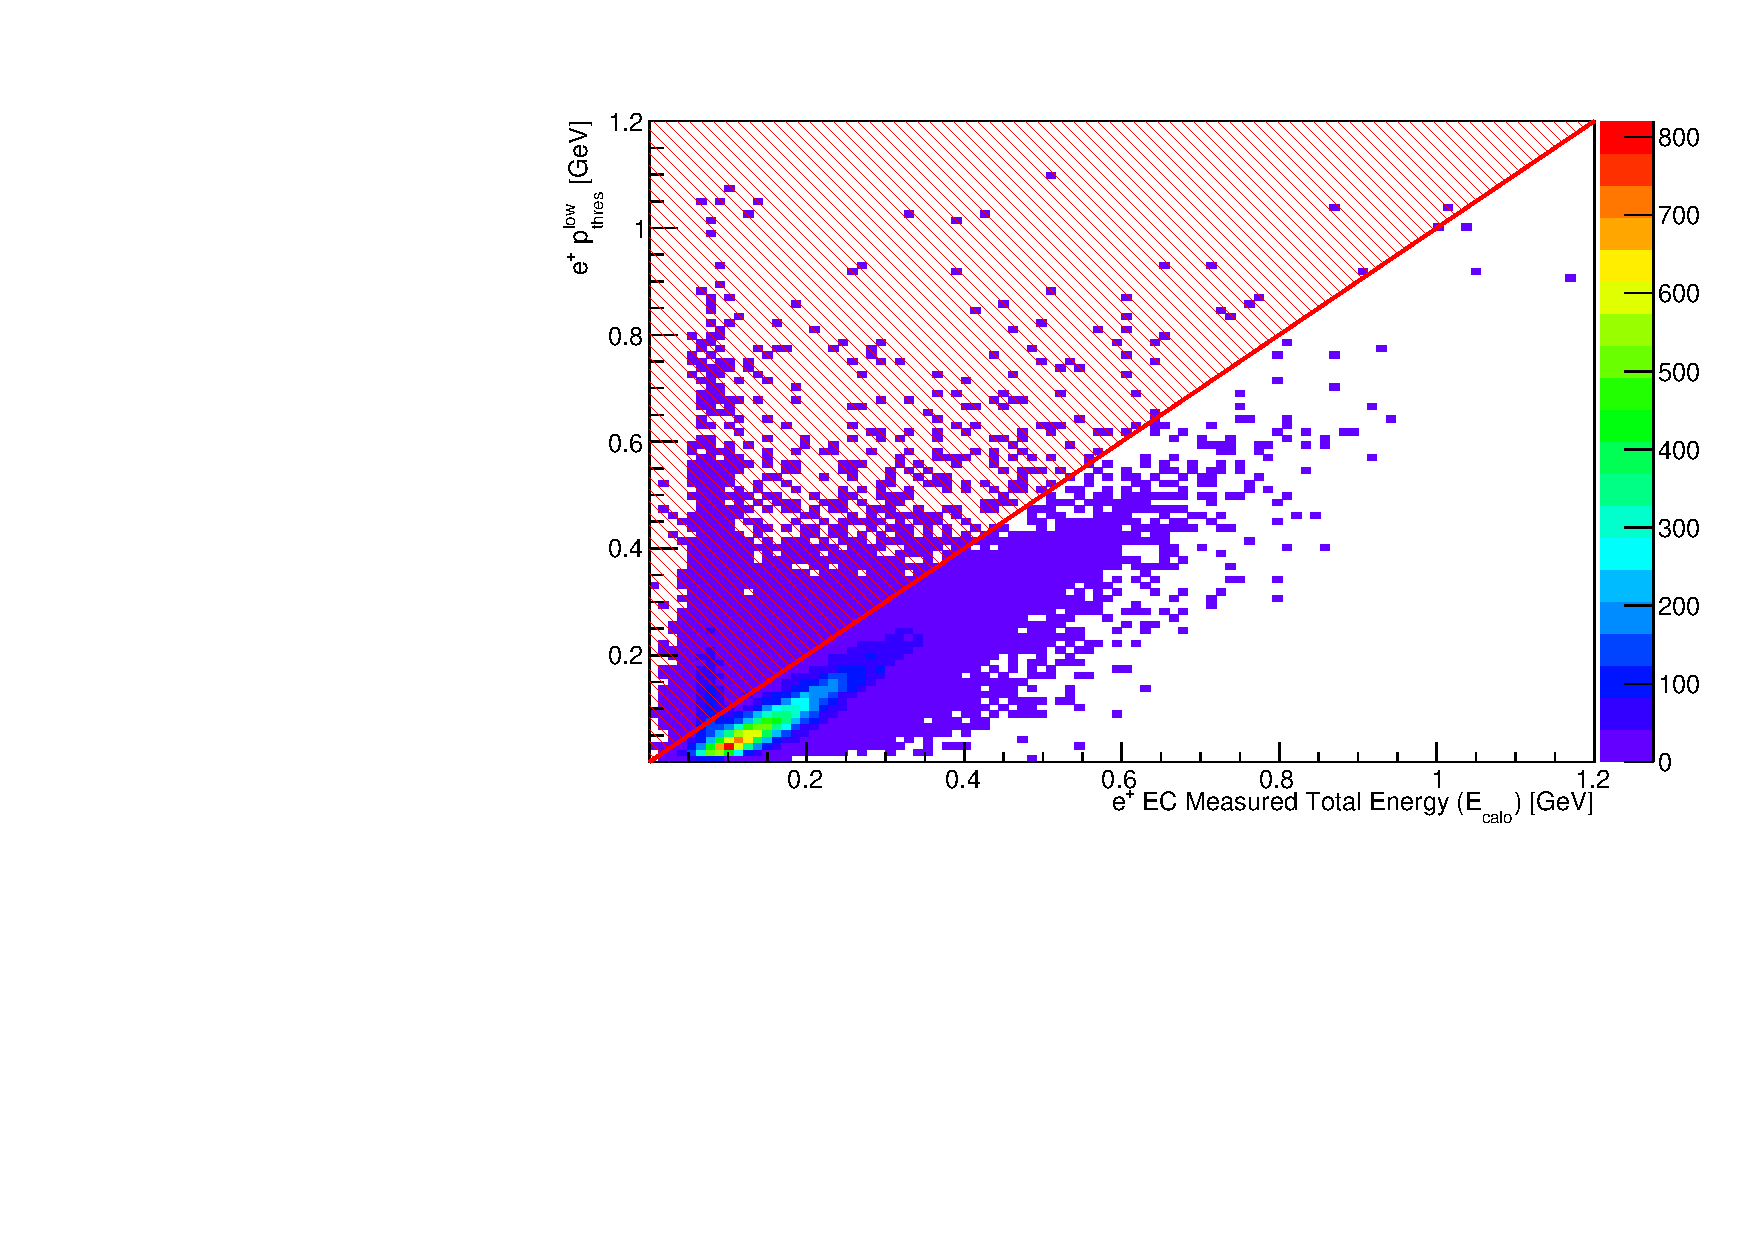
\includegraphics[width=\figwidth,height=0.7\hfigheight]{\figures/analysis/LEP_FEATURES/Pip_EClowcut.pdf}
\caption[\abbr{EC} Deposited Energy Comparison to Track Momentum for e$^+$ Candidates]{\label{fig:islep.pipEC}Plot of energy deposited measured by \abbr{EC} vs. track momentum p$\mathrm{_{thres}^{low}}$ for positrons from \piz events without the \emph{g7} lepton \abbr{EC} \abbr{PID} scheme applied. The red region depicts the cut that would reject events in the \emph{g7} lepton \abbr{EC} \abbr{PID} scheme.}
\end{center}\end{figure}

\begin{figure}[h!]\begin{center}
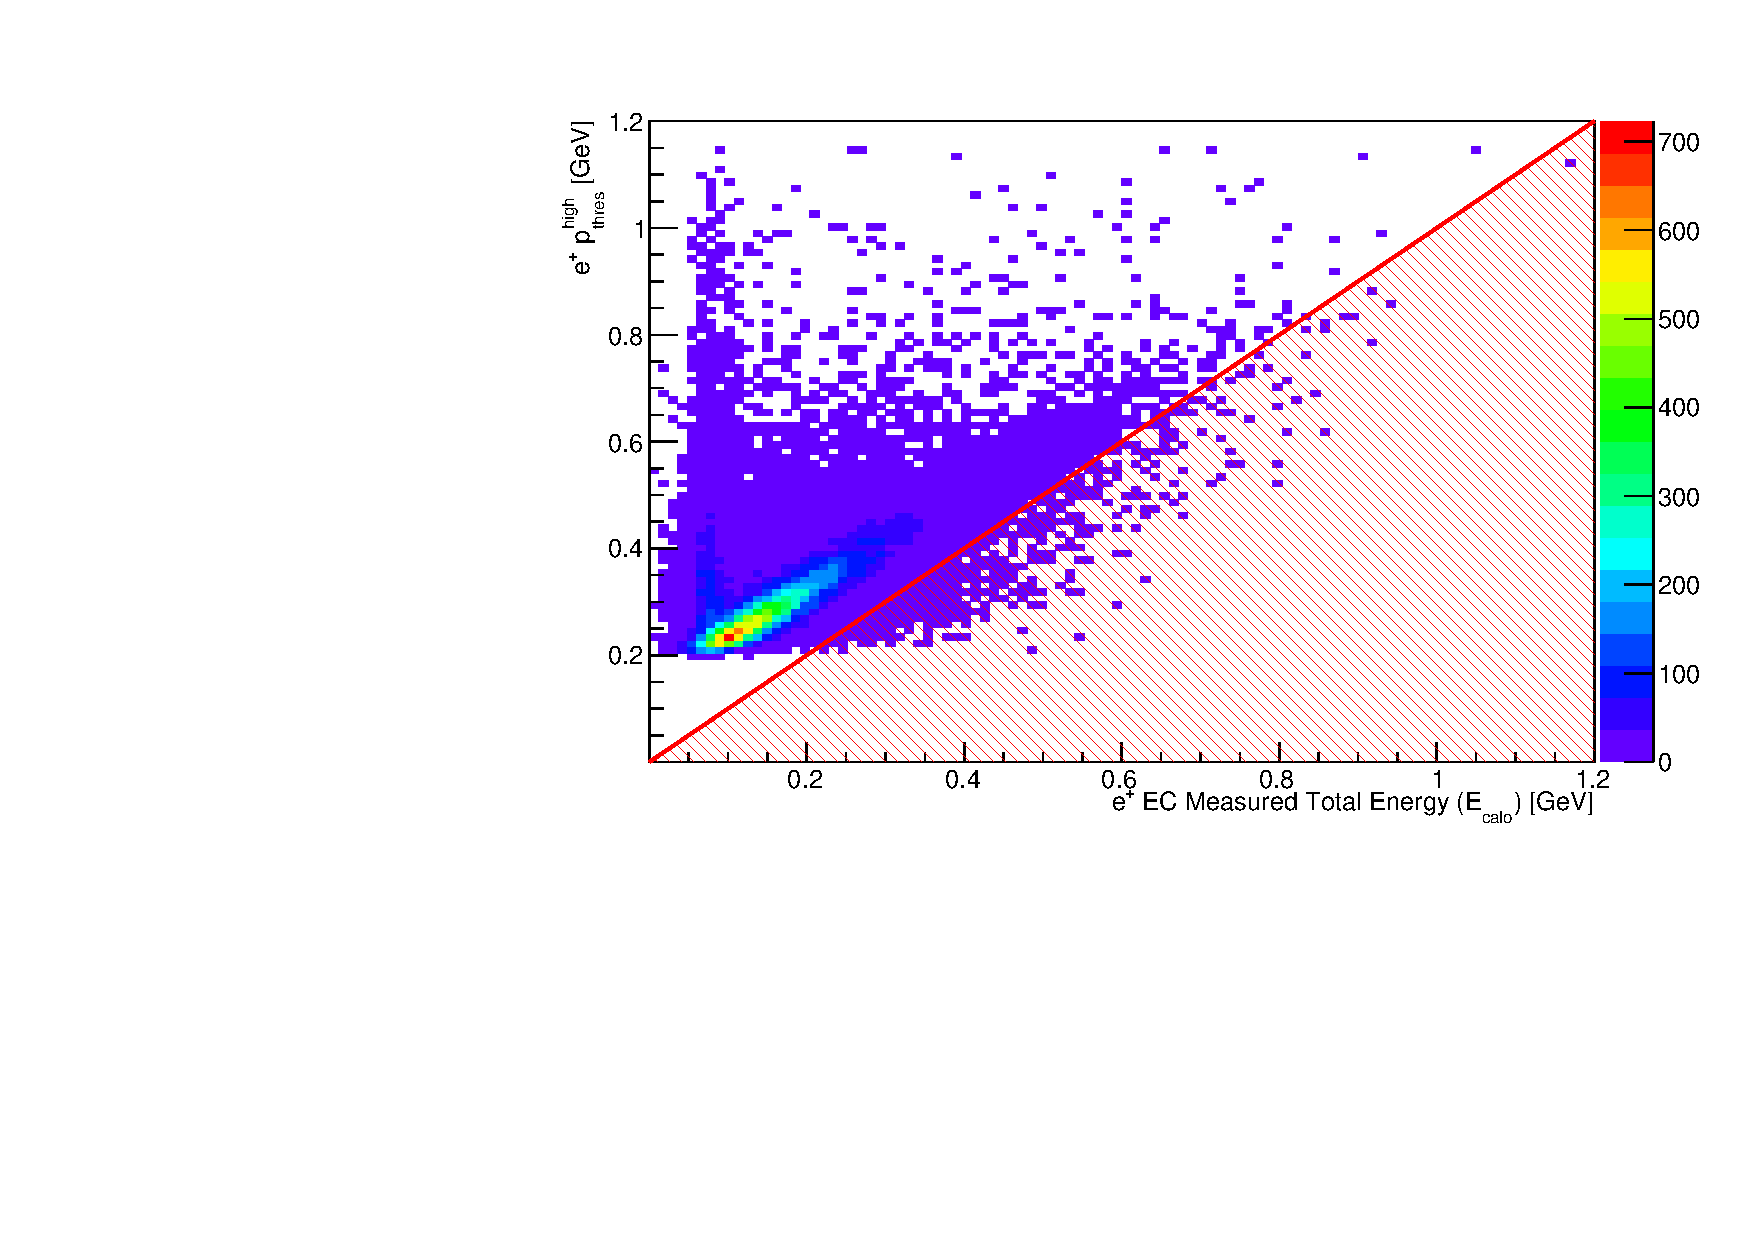
\includegraphics[width=\figwidth,height=0.7\hfigheight]{\figures/analysis/LEP_FEATURES/Pip_EChighcut.pdf}
\caption[\abbr{EC} Deposited Energy Comparison to Track Momentum for e$^+$ from \piz Events]{\label{fig:islep.pipECcut}Plot of energy deposited measured by \abbr{EC} vs. track momentum p$\mathrm{_{thres}^{high}}$ for positrons from \piz events without the \emph{g7} lepton \abbr{EC} \abbr{PID} scheme applied. The red region depicts the cut that would reject events in the \emph{g7} lepton \abbr{EC} \abbr{PID} scheme.}
\end{center}\end{figure}
%


\FloatBarrier



\section{Simulation}\label{sec:analysis.simulation}
There are certain kinematic regions of \abbr{CLAS} in which physics events are not being recorded properly i.e.~the area dividing each sector in \abbr{CLAS}. Furthermore each sector in \abbr{CLAS} is asymmetric in the acceptance of events due to subsystem inefficiencies such as inoperable \abbr{DC} wires, \abbr{PMT} inefficiencies, dead scintillator strips the the \abbr{TOF} and \abbr{ST} subsystems. When a triggered event is recorded and reconstructed these asymmetric inefficiencies factors are reflected and must be carefully understood because these factors are properties of the \abbr{CLAS} detector and independent of any physics that occurred. To properly understand the detector effects on the data, \abbr{CLAS} utilizes a \abbr{GEANT} simulation package know as \abbr{GSIM}. To prepare an event for \abbr{GSIM} the program \abbr{GAMP2PART} converts a text file, containing the 4-momentum of the generated event, into a suitable file format for \abbr{GSIM}. \abbr{GSIM} then simulates the passage of these particles through the \abbr{CLAS} detector and generates the associated \abbr{ADC} and \abbr{TDC} information from detector hits. \abbr{GSIM} takes into account detector inefficiencies described in the \abbr{\texttt{CLAS\_CALDB\_RUNINDEX}}. The \abbr{CLAS\_CALDB\_RUNINDEX} is an array of information about each subsystem's inefficiency that was derived during the \g12 calibration process. The \abbr{GSIM} simulated hits are then ``post-processed'' by smearing the \abbr{TDC} and \abbr{ADC} hits to imitate the observed resolution of the detector subsystems using the program \abbr{GPP} (\abbr{GSIM} post-processor). \abbr{GPP} also removes detector hits due to inefficient \abbr{DC} wires. The simulation output processed with \abbr{GPP} is then reconstructed with \texttt{a1c}, the same program used to reconstruct data events. The reconstructed simulation is subject to the same scrutiny as real data events, undergoing all the cuts (Sec.~\ref{sec:analysis.data.reduction}), corrections (Sec.~\ref{sec:analysis.corrections}), and kinematic fitting (Sec.~\ref{sec:analysis.fitting}), as the real data except for beam corrections (Sec.~\ref{sec:analysis.corrections.beam}).

\subsection{Simulation Verification}\label{sec:analysis.accept.verify}
Part of understanding the simulation output is understanding how well the simulation mimics the real data. To investigate this, 26000 real \epem events were treated as generated events and inputted into the \abbr{GAM2PART}$\to$\abbr{GSIM}$\to$\abbr{GPP}$\to$\texttt{a1c} chain. Of the 26000 inputted, only 100 were successfully reconstructed through the simulation chain. The source of this low efficiency was due to the calibrations entries for the \abbr{CC} and \abbr{EC} in the \abbr{CLAS\_CALDB\_RUNINDEX} not having values in which would set the ``PEDESTAL'' values appropriately for simulation. The calibrations constants in the \abbr{CLAS\_CALDB\_RUNINDEX} were correct for data reconstruction, but not for simulation reconstruction of \epem in the \abbr{CC} and \abbr{EC} subsystems. It was also discovered that the \abbr{CC} and \abbr{EC} subsystems should be simulated with ``RUN 10'' constants instead of the normal ``RUN 56855'' used by the \g12 group. ``RUN 56855'' is a special run benchmarked to have the best calibrations and required to properly simulate the \abbr{ST}, \abbr{DC}, and \abbr{TOF} subsystems. To rectify this, a special \abbr{CLAS\_CALDB\_RUNINDEX} was created, changing ``RUN 10'' for to have ``RUN 56855'' constants for all subsystems except the \abbr{CC} and \abbr{EC} subsystems which were kept at ``RUN 10'' constants. Inputting the 26000 real \epem events into the simulation chain using the \abbr{CLAS\_CALDB\_RUNINDEX} \emph{RunIndexg12\_leptons\_and\_photons} outputted $\approx$~24700 \epem reconstructed events, a $\approx$~95~\% efficiency.

The missing 5~\% was a result of ``time-based'' and ``hit-based'' tracking failures as briefly mentioned in Sec.~\ref{sec:data.cook}. The events that failed ``hit-based'' tracking contributes a 3.75~\% overall event inefficiency. The cause of the ``hit-based'' failure was never determined, but it was thought to have also occur in the cooking of the data. Therefore since it did occur in the data reconstruction this was considered to cancel the inefficiency of the simulation.

The ``time-based'' failure was due to a random bug in the processing of the \abbr{TDC} element information of \abbr{ST} (\abbr{STN0}) and the \abbr{ADC} element information of \abbr{ST} (\abbr{STN1}) raw data banks. The bug miscalculated the tracks sector exiting the \abbr{ST} even as the hit element of the \abbr{ST} matched that to the track in the \abbr{DC}. If the track failed due to this error, it usually passed ``time-based'' on the second or third pass of the ``time-based'' tracking if another particle passed ``time-based'' during the initial pass. The probability that a track failed initial ``time-based" tracking was $\approx$~.23\%. The probability that this failed event would pass ``time-based" tracking after another pass was $\approx99.78\%$. The average inefficiency for three charged track events for data was 0.0125\%

%This inefficiency depends on the distance the track is from the z-vertex position and can be seen in Fig.~\ref{fig:classt.ineffII}.
%\begin{figure}[h!]\begin{center}
%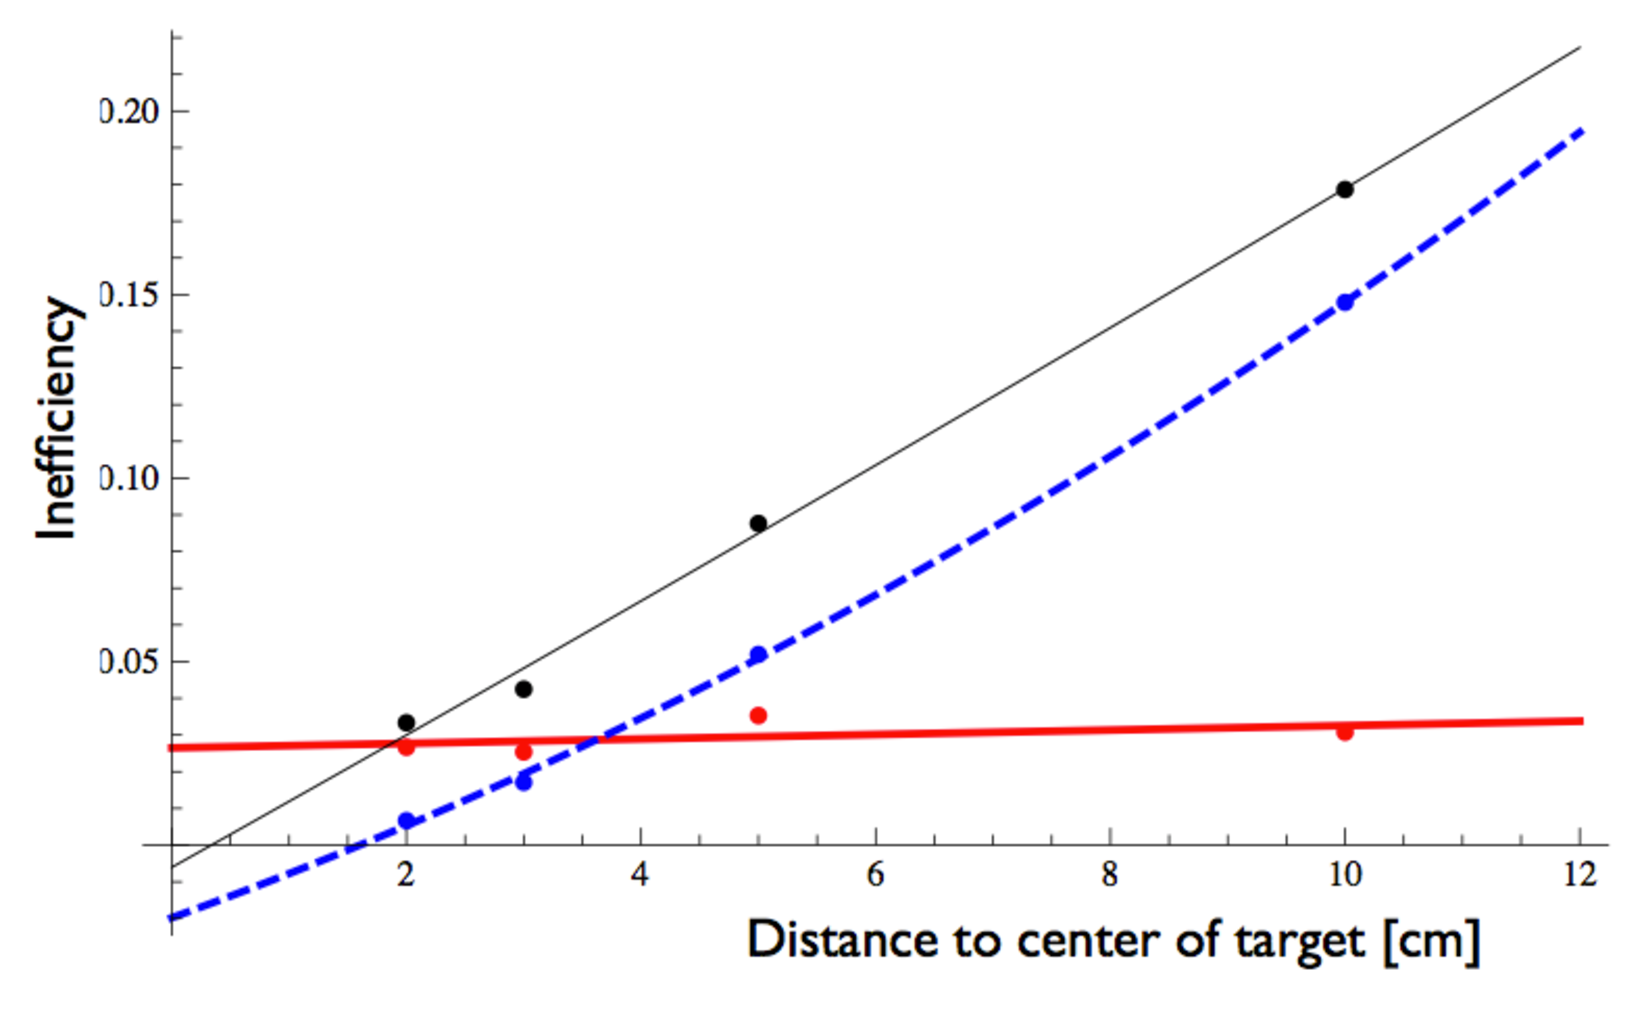
\includegraphics[width=0.8\figwidth,height=0.7\qfigheight]{\grpath/hall-b/st_issue_4_thesis.pdf}
%\caption[Start Counter Inefficiency]{\label{fig:classt.ineffII}{\coloronline}Plot showing the inefficiency of the start counter from data events, red-solid line is the inefficiency of reconstruction based solely on hit-based tracking, blue-dashed line is inefficiency of start counter, black-solid is combined. }
%\end{center}\end{figure}

\FloatBarrier
\subsection{Simulating the Lepton Trigger}\label{sec:analysis.accept.trigger}
During the collection process, for an event to be written by the \abbr{DAQ} it must have passed at least one of the trigger ``bits" defined in Sec.~\ref{sec:clas.g12.conditions.data}. As discussed in Sec.~\ref{sec.data.trig.lepton}, the process of lepton triggering required a coincidence between the \abbr{EC} and the \abbr{CC} subsystems. This coincidence was established by using the voltage sum of the \abbr{CC} for a sector and the voltage sum of the \abbr{EC} for the same sector and comparing each sum to a preset threshold described in Table~\ref{tab:data.ecccthresh}. However when \abbr{GSIM} simulates tracks through the \abbr{CC} and \abbr{EC}, it does not account for the minimum voltage threshold that was required for data collection, moreover the simulation of the trigger must match the trigger efficiency discussed in Sec.~\ref{sec:analysis.trigger.verify}.

Simulation of the \abbr{CC} and \abbr{EC} trigger ``bit 6'', Sec.~\ref{sec.data.trig.lepton}, was performed by writing an algorithm that attempted to mimic the method in which triggered data was recorded. To accomplish this a modified function, written by Simeon McAleer from FSU, was written into the simulation reconstruction algorithm. The routine returned the sector and a boolean of 0 or 1 (pass or fail), that simulated the trigger based on the following criteria;
\begin{enumerate}\label{trig:sim.all}
\item The sector with the highest EC summed energy over threshold. \label{trig:sim.ECtot} 
\item The sector with the highest EC Inner Layer summed energy over threshold. \label{trig:sim.ECinner} 
\item The sector with the highest CC summed energy over threshold. \label{trig:sim.CCtot} 
\item All three above conditions must be in same sector.
\end{enumerate}
Thresholds as described in Table~\ref{tab:data.ecccthresh} are 80~mV, 60~mV and 20~mV for \abbr{EC} \emph{inner}, \abbr{EC}\emph{total} and CC respectively. The \abbr{CC} trigger threshold was applied to groups of eight \abbr{CC} \abbr{PMT}s, called ``sim bits''. The ``sim bits'' were staggered by four \abbr{PMT}s so that each \abbr{PMT} goes into two ``sim bits'', after which all ``sim bits'' were ``\emph{OR}'''d together. If any ``sim bit'' calculated as above threshold, that specific sector was then compared to the remaining sectors to establish the condition listed in~\ref{trig:sim.CCtot}.

The \abbr{EC} \emph{inner} and \abbr{EC} \emph{total} trigger thresholds were applied to all \abbr{EC} strips in a sector. This was done by summing over the energy for every strip in every orientation of the \abbr{EC} per sector. If the energy summation for the \abbr{EC} \emph{inner} was above threshold,   that specific sector was then compared to the remaining sectors to establish the condition listed in~\ref{trig:sim.ECinner}. If the energy summation for the \abbr{EC} \emph{total} was above threshold, that specific sector was then compared to the remaining sectors to establish the condition of the sector with the highest EC summed energy over threshold.

\subsubsection{Validity of Trigger Simulation}
The actual triggered data could have been triggered by the following sceneries;
\begin{enumerate}\label{trig:get.all}
\item $e^-$ \abbr{CC} and \abbr{EC} hit above preset thresholds,
\item $e^+$ \abbr{CC} and \abbr{EC} hit above preset thresholds,
\item $e^-$ \abbr{CC} hit above preset thresholds and $e^+$ \abbr{EC} hit above preset thresholds in the same sector, 
\item $e^-$ \abbr{EC} hit above preset thresholds and $e^+$ \abbr{CC} hit above preset thresholds in the same sector. 
\end{enumerate}
The lepton trigger ``bit 6" was 100\% efficient (see Sec.~\ref{sec:analysis.trigger.verify}) when the data was cut using all the conditions listed above (1, 2, 3, 4) using an ``OR" flag. This means that a $\gamma p \to p e^+ e^-$ event must satisfy at least one of the listed conditions. The reduction in events when at least one of the conditions was satisfied was 69.91\%. Prior to simulating the trigger, cutting the \abbr{MC} with the listed conditions reduced the event yield by 81.91\%. Simulating the trigger and cutting on the \abbr{MC} events with the listed conditions reduced that event yield to 69.48\%. This indicates that the trigger simulation is properly mimicking the trigger configuration used when data is collected. 

%actual physics events recorded by \abbr{CLAS}.
%
%
%When all the conditions listed above are compared together using an ``\emph{OR}'' flag, on \piz data, 69.91\% of events remain. To check the validity of the trigger simulation, events from the \piz reconstructed simulation were placed under the conditions as the actual data. Without placing the boolean of 1 on the simulation, 81.91\% of events remain. Placing the boolean of 1 on the simulation, 69.48\% of events remain, indicating the trigger simulation is mimicking the actual physics events recorded by \abbr{CLAS}. 





\section{PLUTO++ Event Generator}\label{sec:pluto}

Pluto~\cite{PLUTO} is a Monte-Carlo event generator designed for the study of hadronic interactions and heavy ion reactions in \abbr{HADES}, \abbr{FAIR} and upcoming \abbr{PANDA} collaborations. The versatility of Pluto enables its use as an event generator for photoproduction in \abbr{CLAS}. For hadronic interactions, Pluto can generate interactions from pion production threshold to intermediate energies of a few~GeV per nucleon. The entire software package is based on ROOT and uses ROOT's embedded C++ interpreter to control the generation of events. Programming event reaction can be set up with a few lines of ROOT macro code without detailed knowledge of programming. Some features in Pluto are, but not limited to;
\begin{itemize}
\item Ability to generate events in phase space.
\item Ability to generate events with a continuous bremsstrahlung photon beam.
\item Ability to generate events weighted by a user defined $t$-slope.
\item Ability to generate events weighted by a user defined cross-section.
\begin{itemize}
\item Total cross section can be inputted via functional form or histogram.
\item Differential cross sections can be inputted via functional forms or histograms for specific beam energies up to 110 histograms relating to intervals of beam energy.
\end{itemize}
\item Ability to generate events that decay via already established physics parameters, i.e.~transition form factors.
\item Ability to generate events that decay via modified established physics parameters.
\item Ability to generate events with multiple production channels, weighted by user inputted cross-section probability.
\item Ability to generate events with multiple decay channels, weighted by user inputted branching ratio.
\item Ability to perform vertex smearing.
\item Ability to create virtual detectors.
\end{itemize}

For the analysis presented in this work, Pluto was used in conjunction with known differential cross sections to verify simulation momentum smearing and tagger resolution, Sec.~\ref{sec:analysis.simsmear.verify}. Pluto was also utilized as a phase space generator in this analysis, to perform a ``tune'' on the kinematic fitter, Sec.~\ref{sec:analysis.fitting}, to calculate the acceptance corrections Sec.~\ref{sec:results.acceptance}, and to calculate the normalization Sec.~\ref{sec:results.normalization}.
%\section{Particle Vertex Timing Cuts}\label{sec:analysis.timing}
Another quantity that is used for \abbr{PID} and data cleanliness is the vertex timing $t_{vert}$, which is the time the particle left the target. It can be calculated as;
\begin{align}
t_{vert}= t_{\abbr{TOF}} -  l_{\abbr{TOF}}/(c\beta) \label{eq:tvert.tof}
\end{align}
where $t_{\abbr{TOF}}$ and $l_{\abbr{TOF}}$ are the time and length measurement, respectively, recorded at the \abbr{TOF} subsystem, and $c$ is the speed of light. The value of $\beta$ is calculated using the particles mass, $m$, and momentum, $p$, as measured from the \abbr{DC}. Therefore $\beta = \frac{p}{E} = \frac{p}{\sqrt{p^2+m^2}}$. Another means of calculating $t_{vert}$ is to use the timing of the tagger hit using the RF-corrected tagger time, see tagger calibration in \cite{clas.g12.note}. In this method $t_{vert}$ is calculated as;
\begin{align}
t_{vert}=t_{pho} + t_{prop} \label{eq:tvert.tagger}
\end{align}
where $t_{pho}$ is the RF-corrected time that the photon crossed the center of the target and $t_{prop}$ is the propagation time from the center of the target to the track's vertex. Comparing the two quantities of $t_{vert}$ from Eq.~\ref{eq:tvert.tof} and Eq.~\ref{eq:tvert.tagger} gives information of proper particle timing as well as the \abbr{PID}. In Fig.~\ref{fig:timing.all}, the comparison of the difference $t_{(vert, \ tagger)} - t_{(vert,\ \abbr{TOF})}$ is shown for the detected proton, $e^-$, and $e^+$ for data and \abbr{MC} after all geometric, \abbr{TOF}, \abbr{EC} fiducial cuts as well as all analysis cuts mentioned previously. A cut of $\pm 1.2$~ns was placed on all particles, the effect is minimal.

%Sec.~\cref{sec:analysis.fid_cuts}, Sec.~\ref{sec:analysis.tof_fid}, Sec.~\ref{sec:analysis.eccc_fid} and Sec.~\ref{sec:analysis.analysis_cuts}.

\begin{figure}[h!]\begin{center}
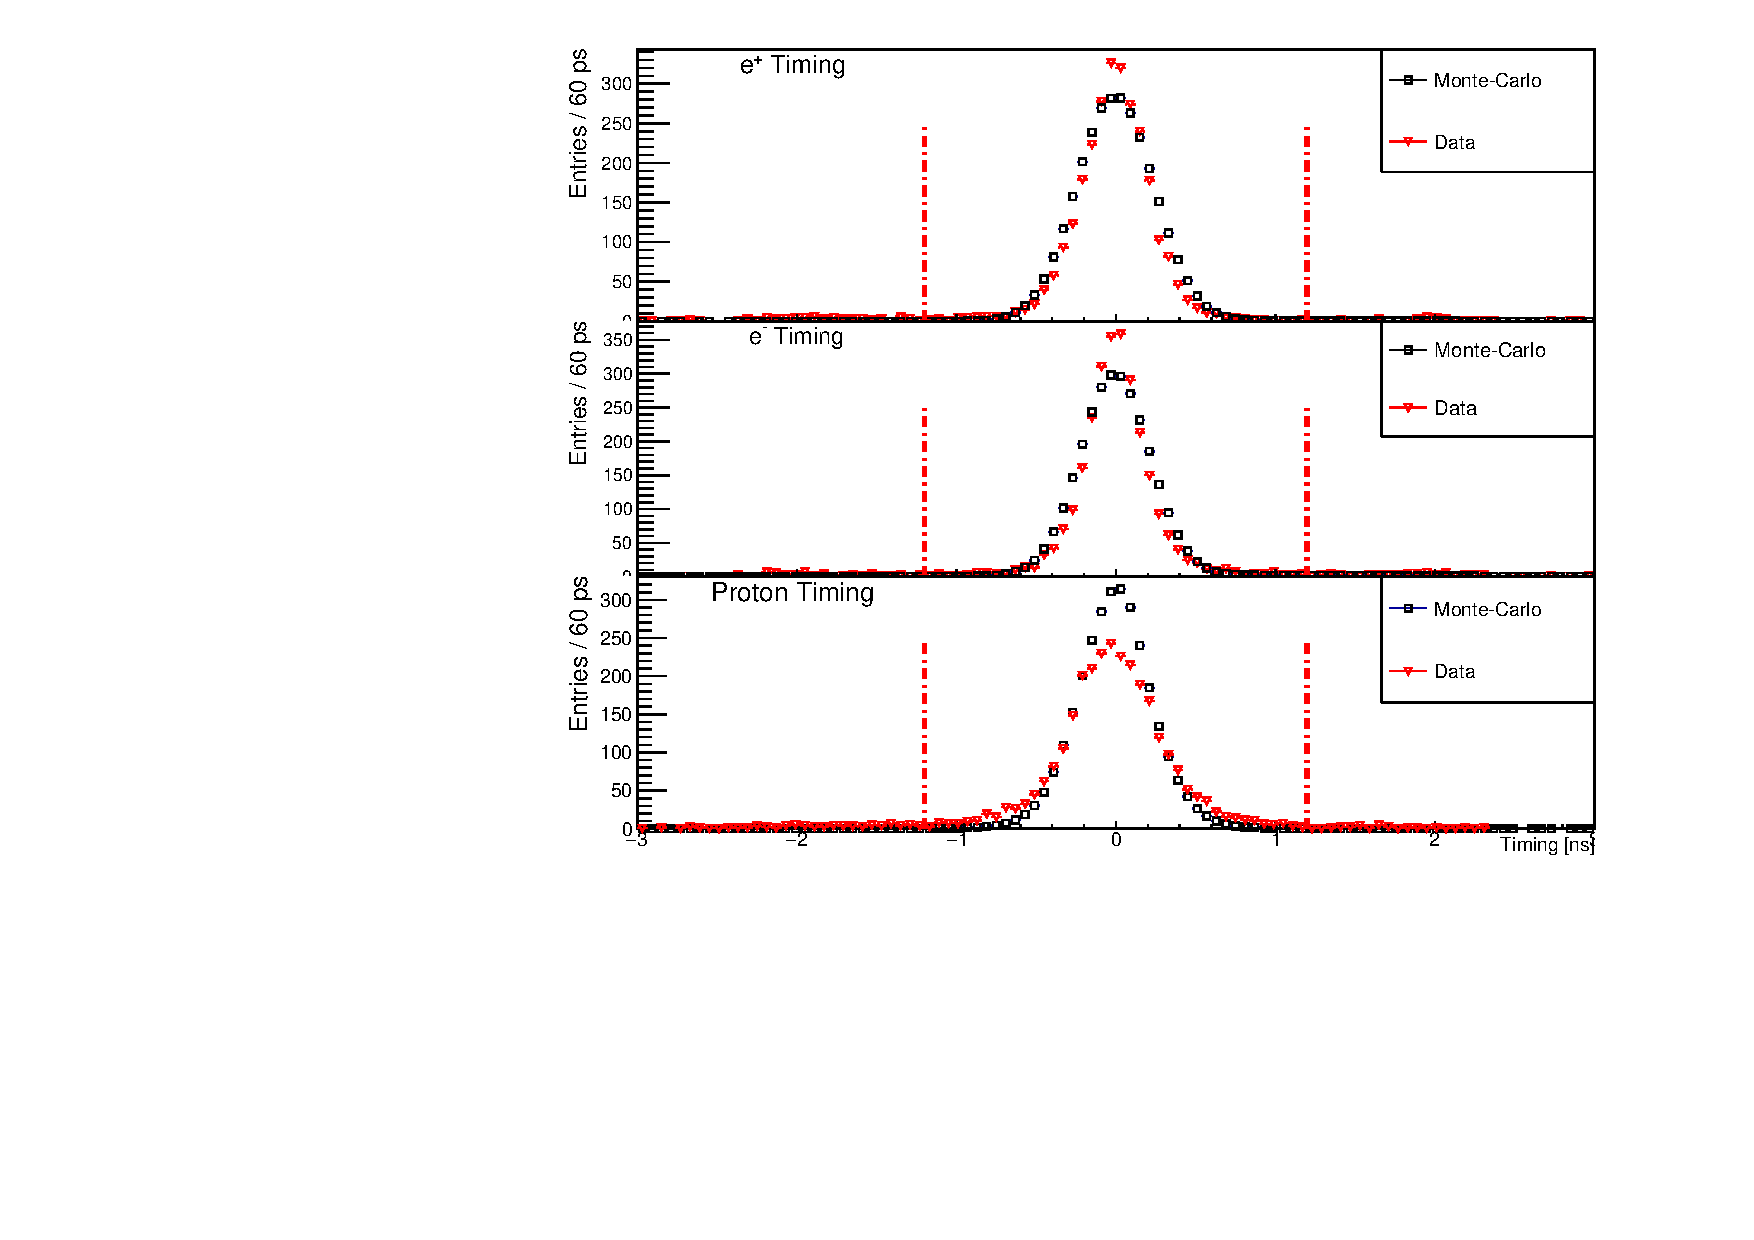
\includegraphics[width=\figwidth,height=\hfigheight]{\figures/analysis/TIMING/Timing_Plots.pdf}
\caption[Number of events vs. $t_{pho} + t_{prop} - (t_{\abbr{TOF}} -  l_{\abbr{TOF}}/(c\beta))$ for \abbr{MC} and data for proton, $e^-$, and $e^+$]{\label{fig:timing.all}Number of events vs. $t_{pho} + t_{prop} - (t_{\abbr{TOF}} -  l_{\abbr{TOF}}/(c\beta))$ for \abbr{MC} and data for proton, $e^-$, and $e^+$.}
\end{center}\end{figure}

\FloatBarrier
\section{$z$ Vertex Cuts}\label{sec:analysis.zvert}
To ensure that \pizT production occurred on the $\ell$H$_2$ target, a cut was placed on the $z$-vertex position to be $-110 \le z \le -70$ (see Fig.). Since the vertex resolution of \abbr{CLAS} is 1~cm, there is a probability of \pizT production on the Kapton endcaps of the target. This effect was studied as a systematic uncertainty (see Sec~\ref{sec:results.systematics}). 
\begin{figure}[h!]\begin{center}
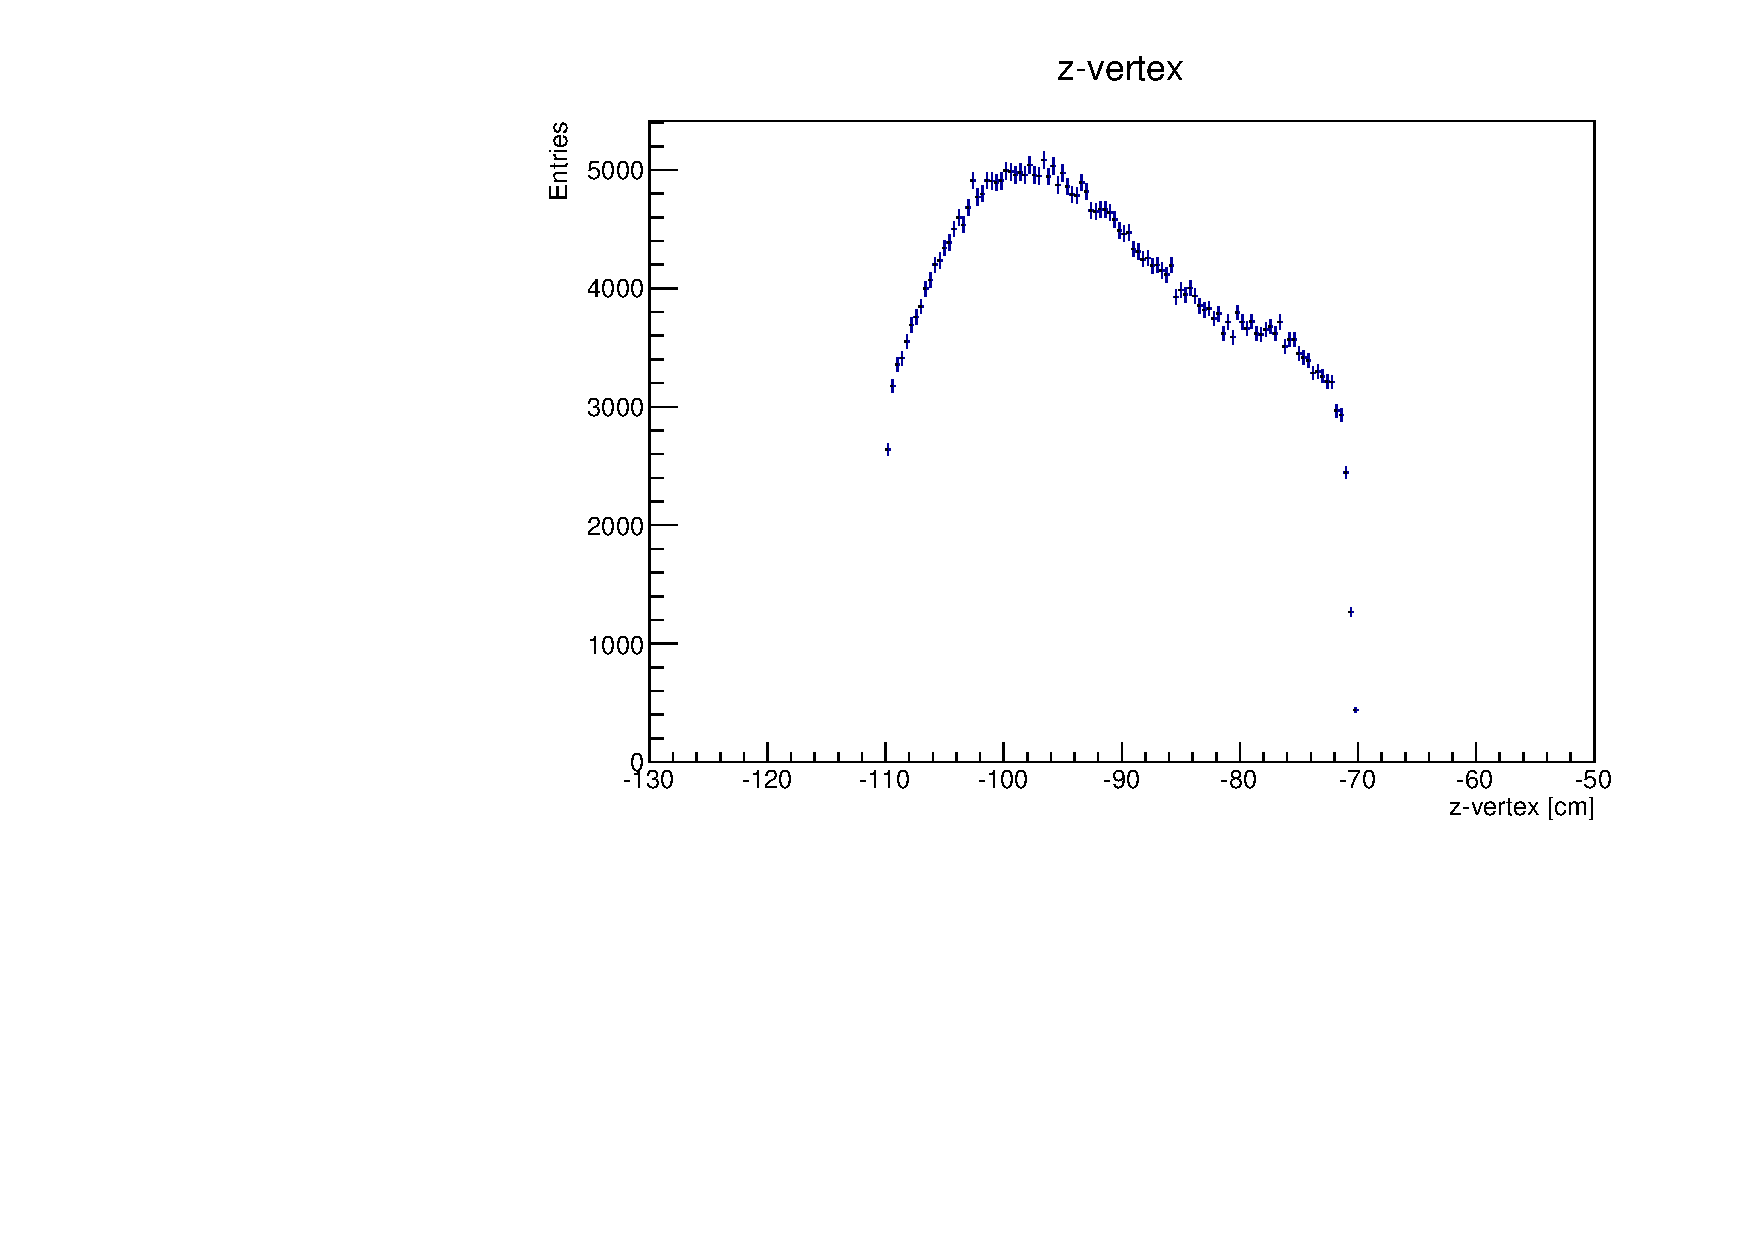
\includegraphics[width=\figwidth,height= 0.75 \hfigheight]{\figures/analysis/TARGET_DENSITY/z-vertex.pdf}
\caption[Number of data events plotted vs. $z$-vertex]{\label{fig:zcut}Number of data events plotted vs. $z$-vertex}
\end{center}\end{figure}
The z-vertex is not flat because of acceptance. At large angles(backward) the acceptance in \g12 was reduced to $\approxeq$100 degrees for single particle detection. For multi-particle detection, the acceptance, at large angles, was reduced to $\approxeq$70 degrees (see Fig.~\ref{fig:Ptheta_z}). For particles that originated from the start of the target, this acceptance effect was prominent. For $\pi^0$ production in \g12, in which the decay of $\pi^0$ was identified with \epem($\gamma$) events, the acceptance was largest when production occurred near the center of the target. When production happened in the forward part of the target, the dilepton acceptance was reduced. 

\begin{figure}[h!]\begin{center}
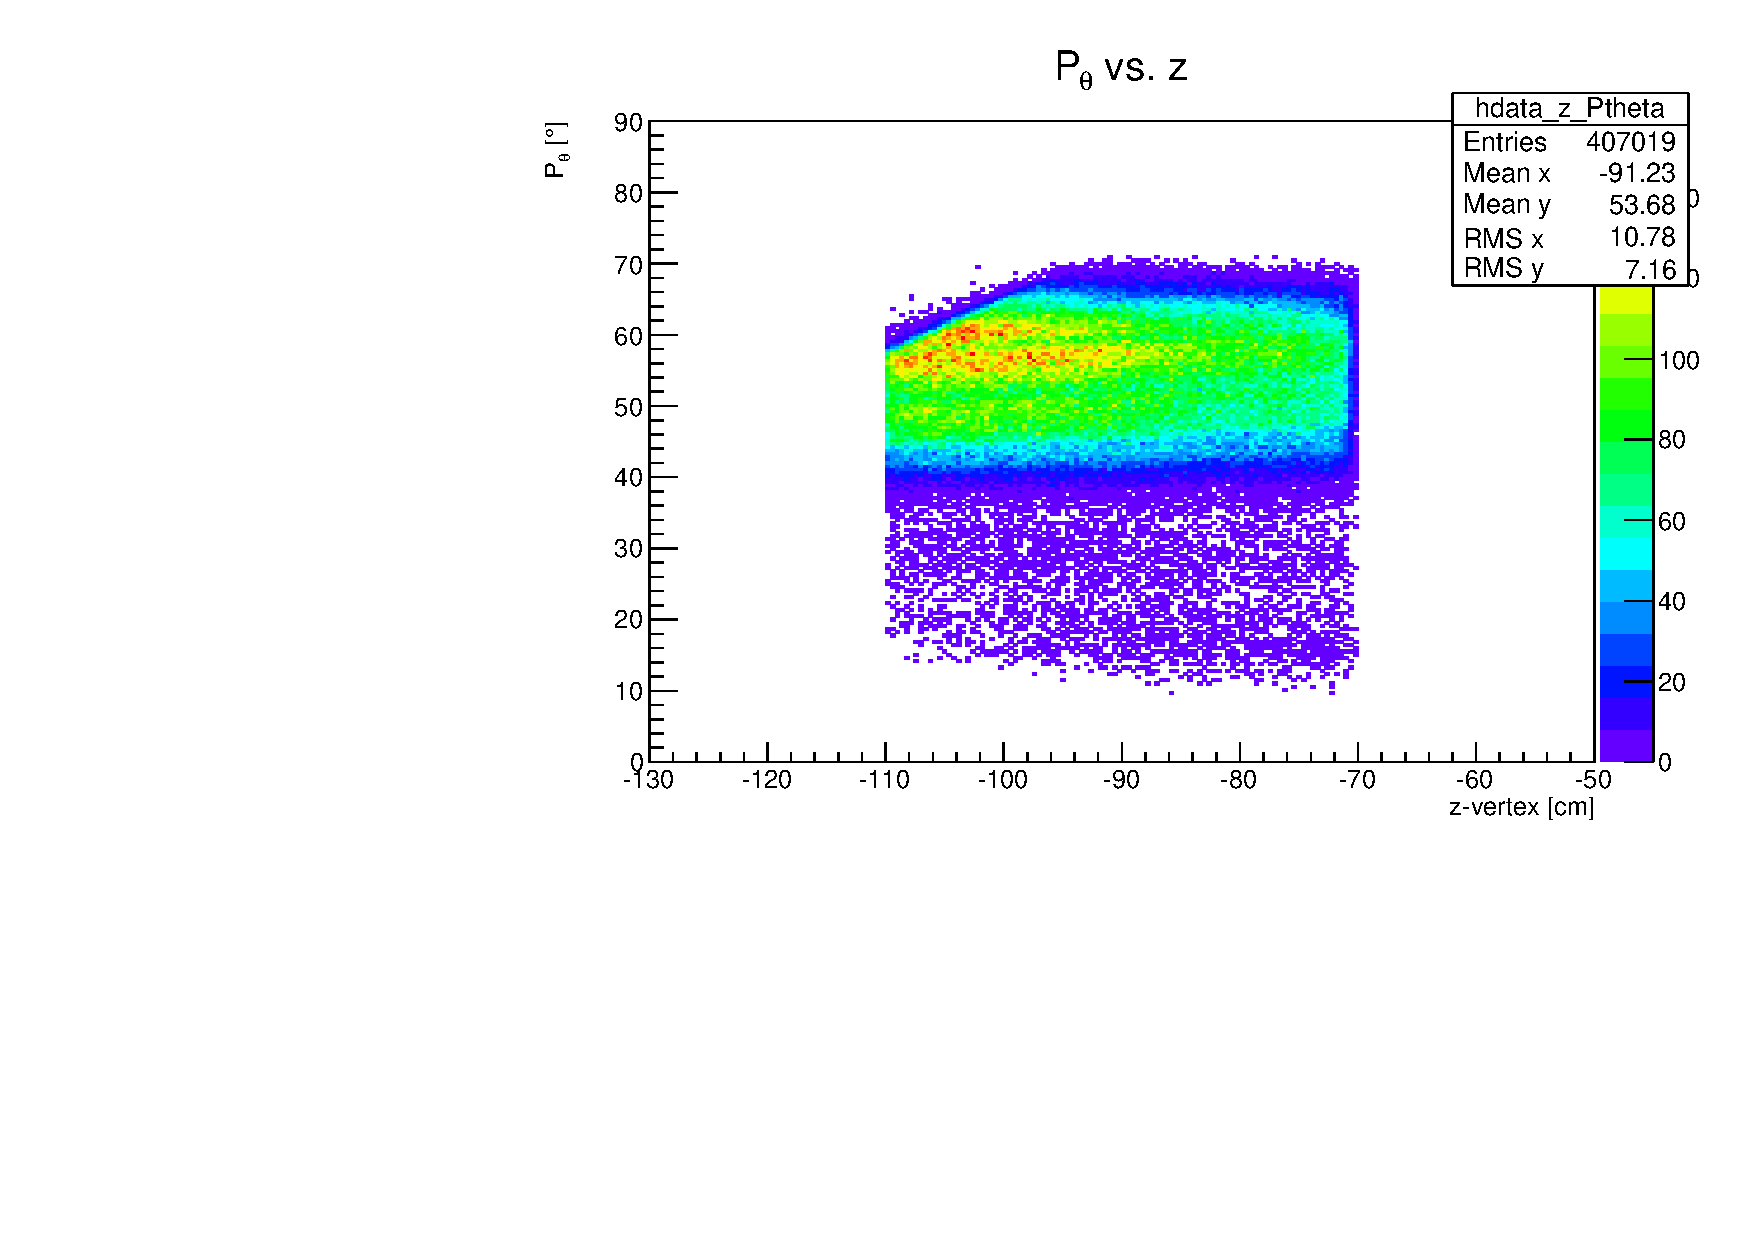
\includegraphics[width=\figwidth,height= 0.75 \hfigheight]{\figures/analysis/TARGET_DENSITY/PTheta_vs_z.pdf}
\caption[Proton $\theta$ vs. $z$-vertex]{\label{fig:Ptheta_z}Proton $\theta$ vs. $z$-vertex. The z-axis depicts the total number of events.}
\end{center}\end{figure}
\FloatBarrier
\subsubsection{Final Data Distribution}\label{sec.final.data}
The final data selection used for measuring of physics variables from \pizT production for this analysis can be seen in Fig.~\ref{fig:kinfit.final.plot}.

\begin{figure}[h!]\begin{center}
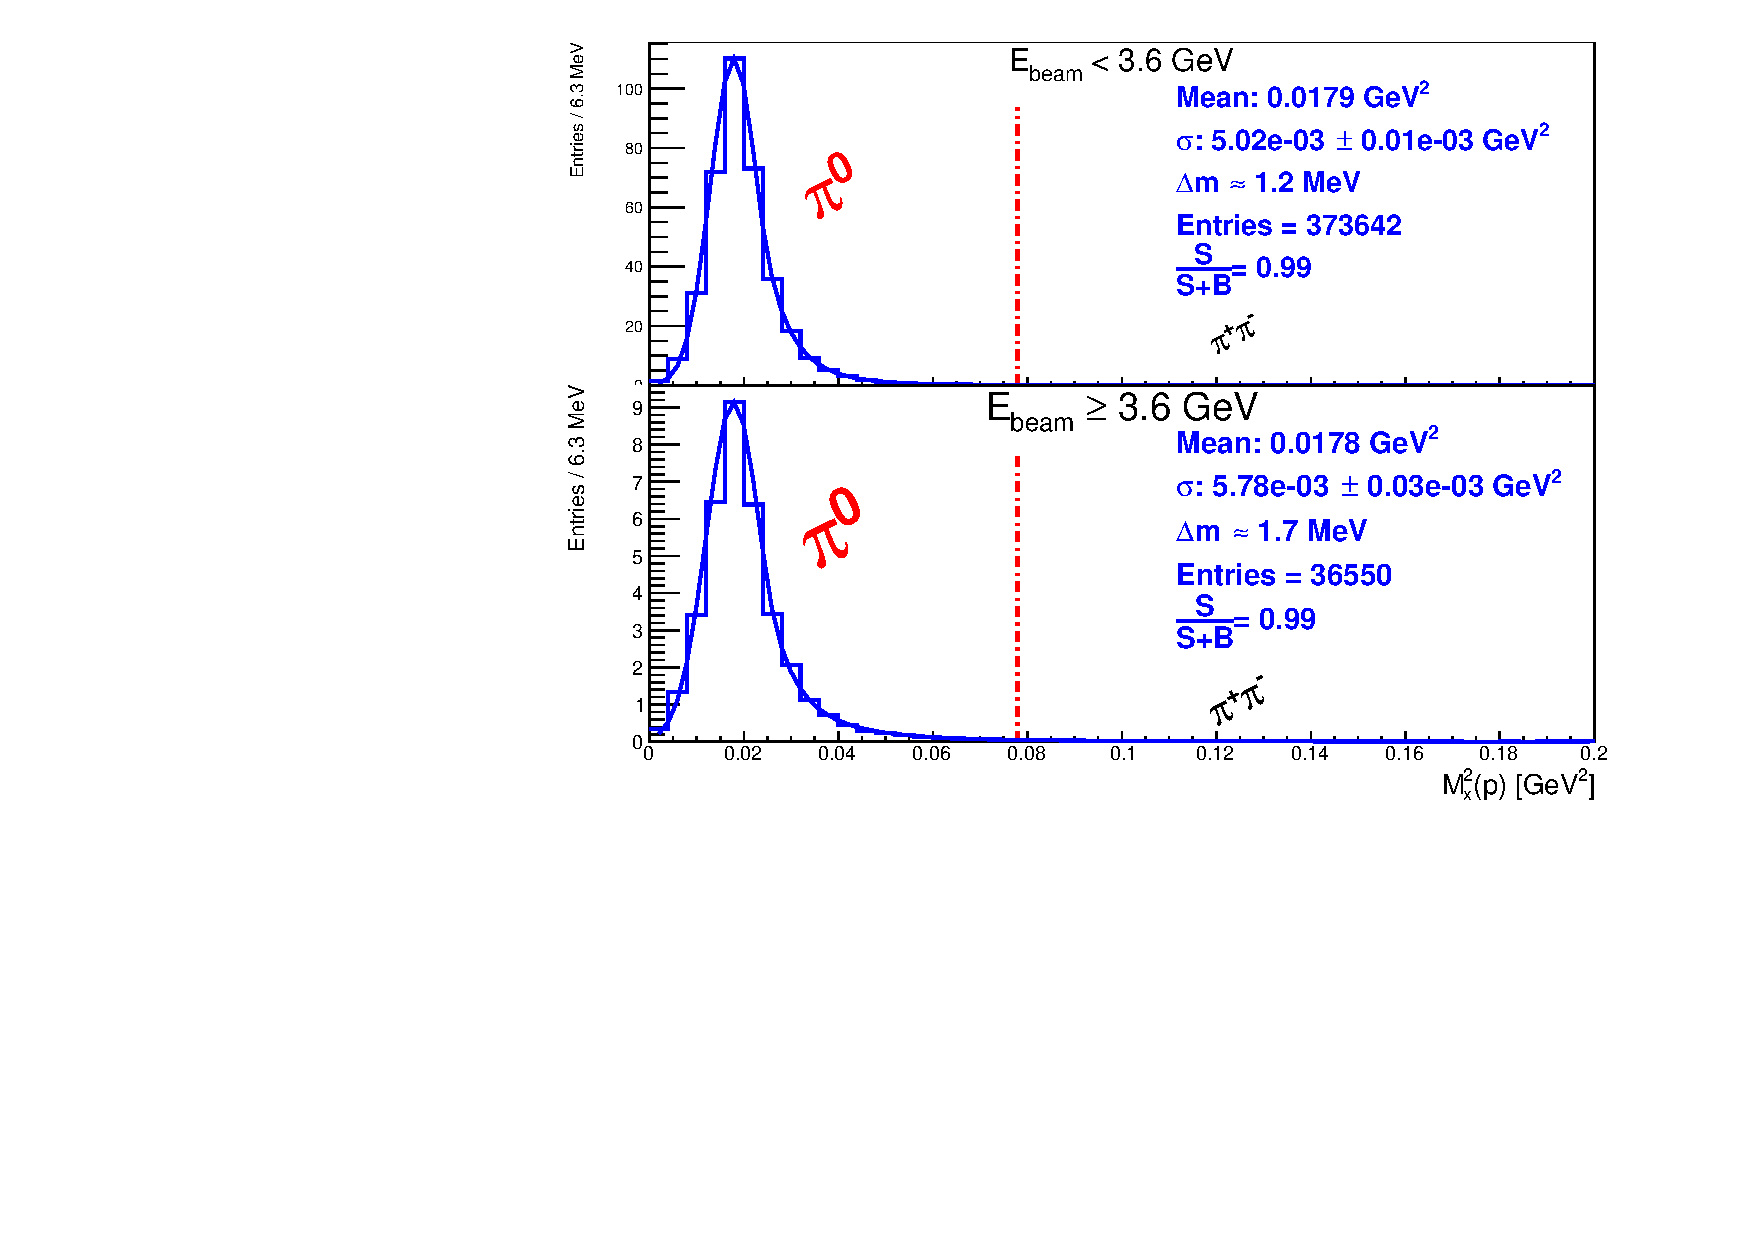
\includegraphics[width=\figwidth,height= 0.75 \hfigheight]{\figures/analysis/KineFitter/DATA/hdataLEP_MOR_pi0_FINAL_PLOTS.pdf}
\caption[Number of data events plotted vs. missing mass $M_x(\gamma p \to p X)$ for $\gamma p \to p e^+ e^- (\gamma)$ events after all cuts and corrections.]{\label{fig:kinfit.final.plot}Number of data events plotted vs. missing mass $M_x(\gamma p \to p X)$ for $\gamma p \to p e^+ e^- (\gamma)$ events after all cuts and corrections.}
\end{center}\end{figure}
\FloatBarrier

%\subsection{Beam Photon Identification}\label{sec:analysis.beam}

As described in Sec.~\ref{sec:analysis.excluded}, only runs in which the beam current was 60-65~nA were used. This high current incident on the radiator can create multiple tagger hits within the time gate of the trigger. To determine which beam photon interacted with the target creating the event, a tagger time best matching the average \abbr{ST} time is chosen to be the time of the interacting photon that created the triggered event.

Due to the 2.004~ns \abbr{CEBAF} beam bunching spacing, there are possibilities in which a beam bunch will contain multiple bremsstrahlung photons that are indistinguishable in timing, within 2.004~ns, that satisfy the best tagger time. Figs~\ref{fig:beam.timing} and~\ref{fig:beam.timingII} show that $\simeq$ 86\% of events have a single in-time tagger-\abbr{ST} coincidence, $\simeq$ 11.5\% of events have two in-time tagger-\abbr{ST} coincidences, $\simeq$ 2\% of events have three in-time tagger-\abbr{ST} coincidences and $<$ .5\% of events have have more than three in-time tagger-\abbr{ST} coincidences. For the events in which there are multiple photons within the 2.004~ns window that are in time with the \abbr{ST}, the best photon is chosen at random with no preference to the energies of each photon. This method of random choice allows for a 7\% background increase due to the mismatching of the photon The 7\% is due to randomly choosing the incorrect photon $\frac{1}{2}$ of the 14\%. 

\begin{figure}[h!]\begin{center}
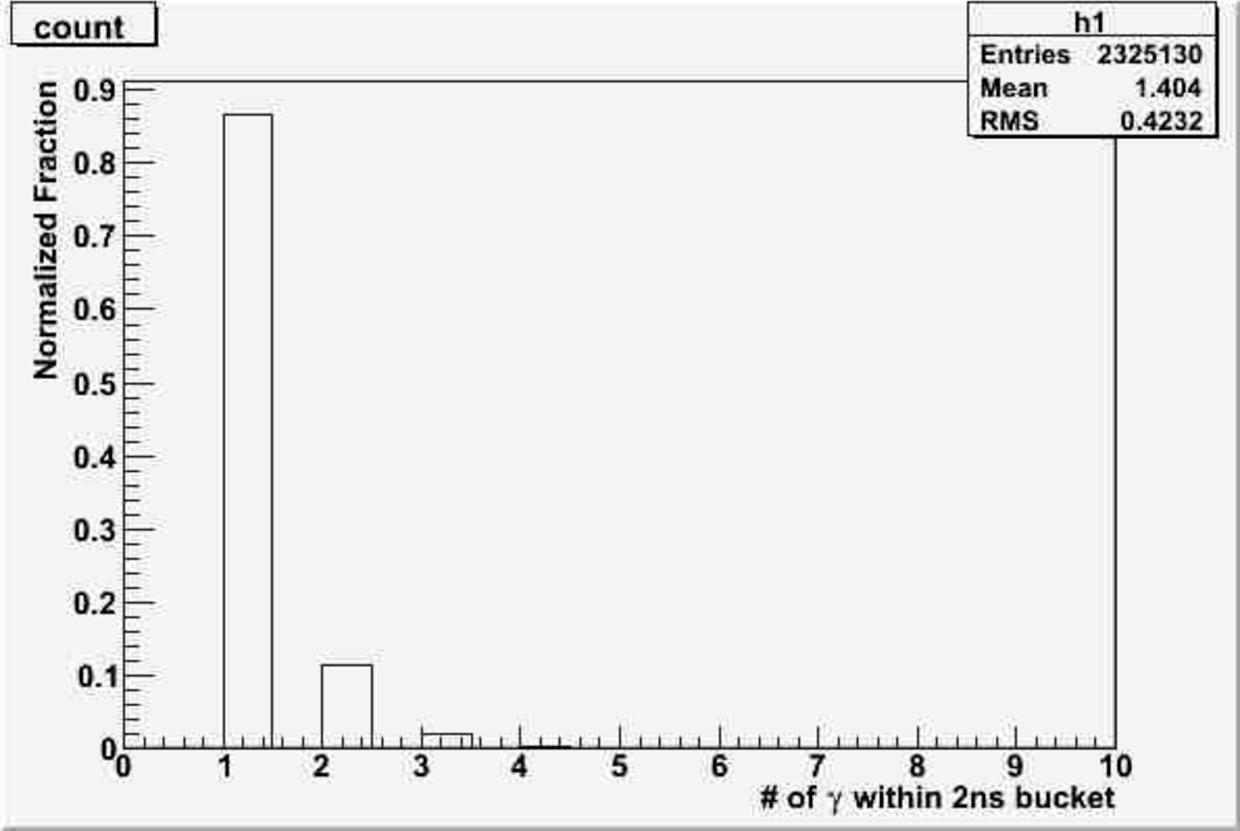
\includegraphics[width=\figwidth,height=0.75\hfigheight]{\figures/analysis/photon_timing/Photoncount1.pdf}
\caption[Probability of single and multiple photons within the \abbr{CEBAF} timing window of 2.004~ns]{\label{fig:beam.timing}Probability of single and multiple photons within the \abbr{CEBAF} timing window of 2.004~ns.}
\end{center}\end{figure}

\begin{figure}[h!]\begin{center}
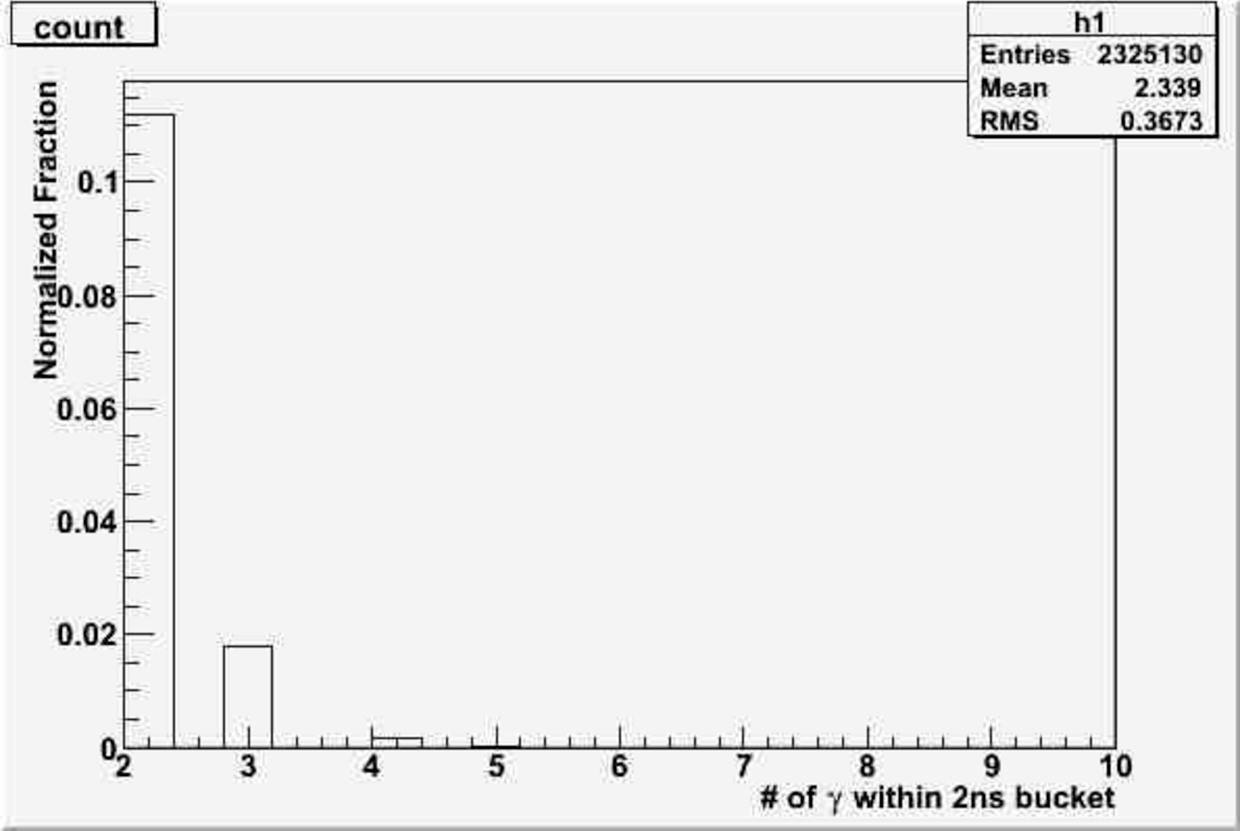
\includegraphics[width=\figwidth,height=0.75\hfigheight]{\figures/analysis/photon_timing/Photoncount.pdf}
\caption[Probability of multiple photons within the \abbr{CEBAF} timing window of 2.004~ns]{\label{fig:beam.timingII}Probability of multiple photons within the \abbr{CEBAF} timing window of 2.004~ns.}
\end{center}\end{figure}

\FloatBarrier
%\chapter{\label{sec:app.tofe}\abbr{TOF} Energy Deposit Cut}

Listed below is a summary of the time-of-flight energy deposit cuts where $p$ is the momentum of the particle in GeV, and the energy deposit, $\frac{\Delta E}{\Delta x}(\mathtt{TOF})$, is in units of MeV/cm. Each cut consists of a linear part applied below a certain momentum and a $p^{-2}$ part above this momentum.

\begin{itemize}
    \item[] protons:
    \begin{itemize}
        \item[] $p > 0.4$~GeV
        \begin{itemize}
            \item[] $\frac{\Delta E}{\Delta x}(\mathtt{TOF}) > 1.45 + \frac{1}{0.4 (p - 0.07)^2}$~MeV/cm
            \item[] $\frac{\Delta E}{\Delta x}(\mathtt{TOF}) < 2.70 + \frac{1}{0.9 (p - 0.15)^2}$~MeV/cm
        \end{itemize}
        \item[] $p \leq 0.4$~GeV
        \begin{itemize}
            \item[] $\frac{\Delta E}{\Delta x}(\mathtt{TOF}) > 59 p - 14.5$~MeV/cm
            \item[] $\frac{\Delta E}{\Delta x}(\mathtt{TOF}) < 59 p - 10.0$~MeV/cm
        \end{itemize}
    \end{itemize}
    \item[] pions:
    \begin{itemize}
        \item[] $p > 0.08$~GeV
        \begin{itemize}
            \item[] $\frac{\Delta E}{\Delta x}(\mathtt{TOF}) > 1.3 + \frac{1}{40 (p + 0.02)^2}$~MeV/cm
            \item[] $\frac{\Delta E}{\Delta x}(\mathtt{TOF}) < 2.5 + \frac{1}{ 8 (p + 0.03)^2}$~MeV/cm
        \end{itemize}
        \item[] $p \leq 0.08$~GeV
        \begin{itemize}
            \item[] $\frac{\Delta E}{\Delta x}(\mathtt{TOF}) > 0$~MeV/cm
        \end{itemize}
    \end{itemize}
    \item[] kaons:
    \begin{itemize}
        \item[] $p > 0.22$~GeV
        \begin{itemize}
            \item[] $\frac{\Delta E}{\Delta x}(\mathtt{TOF}) > 1.5 + \frac{1}{ 3 (p + 0.05)^2}$~MeV/cm
            \item[] $\frac{\Delta E}{\Delta x}(\mathtt{TOF}) < 2.6 + \frac{1}{ 4 (p + 0.12)^2}$~MeV/cm
        \end{itemize}
        \item[] $p \leq 0.22$~GeV
        \begin{itemize}
            \item[] $\frac{\Delta E}{\Delta x}(\mathtt{TOF}) > 59 p - 7$~MeV/cm
            \item[] $\frac{\Delta E}{\Delta x}(\mathtt{TOF}) < 59 p$~MeV/cm
        \end{itemize}
    \end{itemize}
\end{itemize}

%\input{analysis/mmkk}
